In this section, we document the results on the upper-limits using shape analysis based on 
the matrix element output, described in Section~\ref{sec:LR}. 
%The matrix element output has been evaluated for 18 different values of $m_H$ between 115 and 600 \GeVcc.
Figure~\ref{fig:me_115_4700pb}-\ref{me_200_4700} shows the likelihood ratio distributions for $m_H$~=~115, 120, 130, 140, 160 and 200\GeVcc,               
corresponding to 4.7~fb$^{-1}$. 
Note that the majority of backgrounds peak near $LR~=~0$ while the signal peaks near $LR~=~1$.  
It was noted in Sec.~\ref{sec:EvtSelWW} that we apply a dilepton invariant mass requirement prior to constructing the likelihood ratio. 
Figure~\ref{fig:LR_noMll} shows the likelihood ratio distribution assuming $m_{H}=160$ \GeVcc without the invariant mass requirements.
One can see from the peak at $LR~=~0$ that the Matrix Element method successfully identifies high invariant mass events as background-like, so the cut is not essential. However, by applying the cut we lose less than $1\%$ of the signal and gain significantly in processing time needed for differential cross-section calculations.

%%%%%%%%%%%%%%%%%%%%%%%%%%%%%%%%%%%%%
\begin{figure}[!hbtp]                                                                                         
\centering                                                                                                                                             
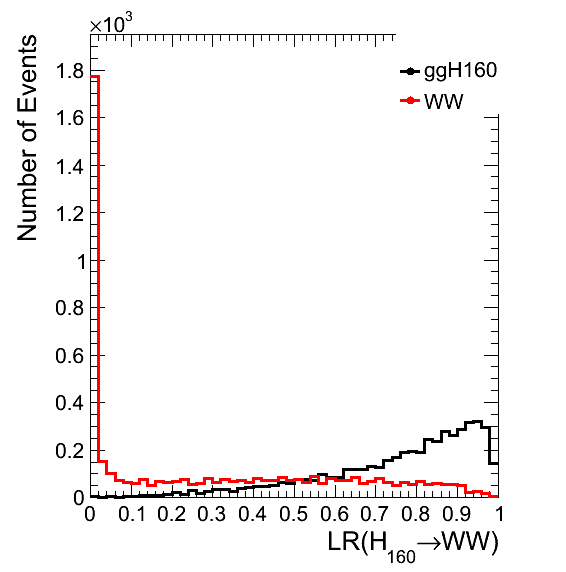
\includegraphics[width=.5\textwidth]{figures/LR_noMll.png}\\                                            
\caption{The matrix element output LR distribution after $WW$ selection but prior to $m_{ll}$ cut                      
for $m_H$=160 \GeVcc}
\label{fig:LR_noMll}                                                                                          
\end{figure}
%%%%%%%%%%%%%%%%%%%%%%%%%%%%%%%%%%%%%




%%%%%%%%%%%%%%%%%%%%%%%%%%%%%%%%%%%%%
\begin{figure}[!hbtp]
\centering
\subfigure[$e\mu$ 0-Jet]{
\centering
\label{subfig:me_115_0j_of_4700pb}
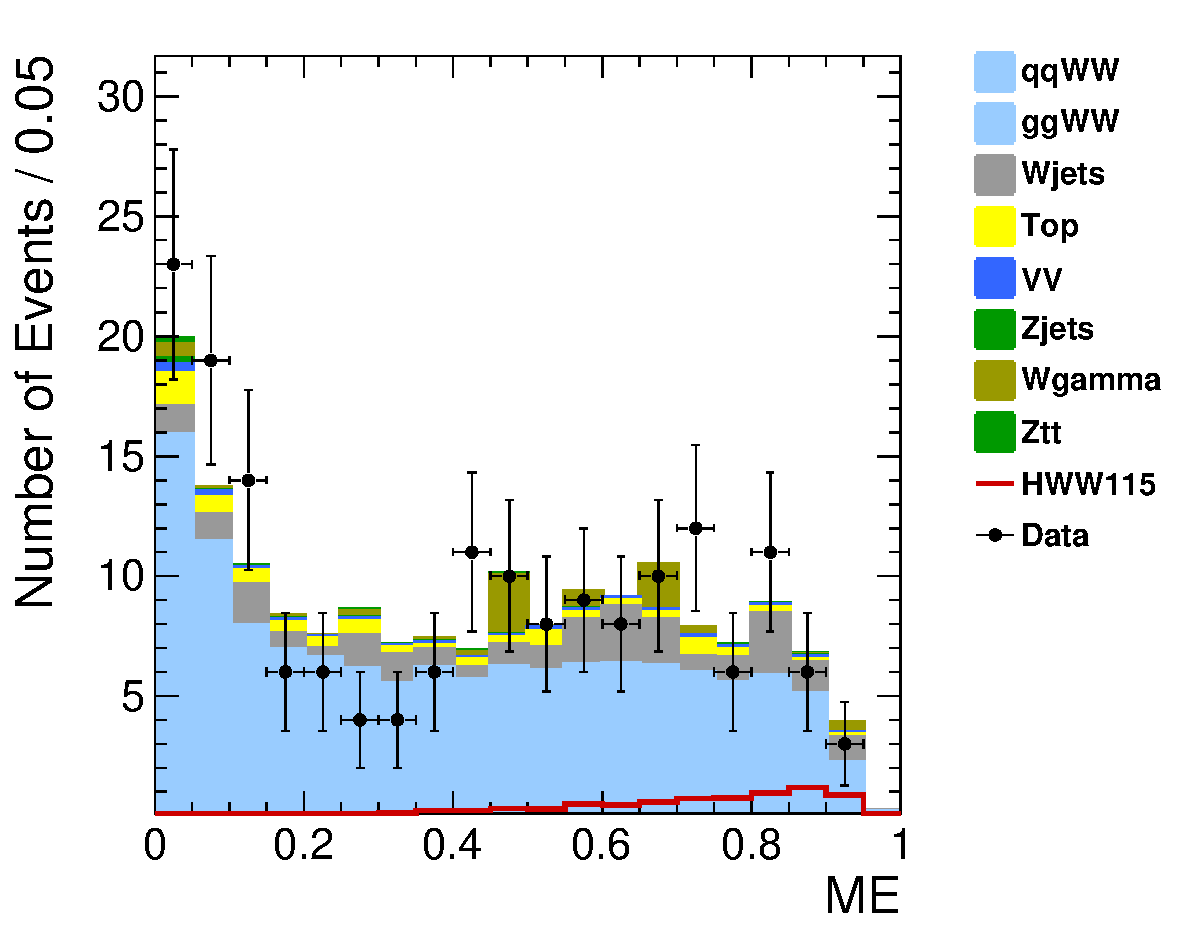
\includegraphics[width=.40\textwidth]{figures/ME_mH115_0j_of_stack_lin.pdf}}
\subfigure[$ee$/$\mu\mu$ 0-Jet]{
\centering
\label{subfig:me_115_0j_sf_4700pb}
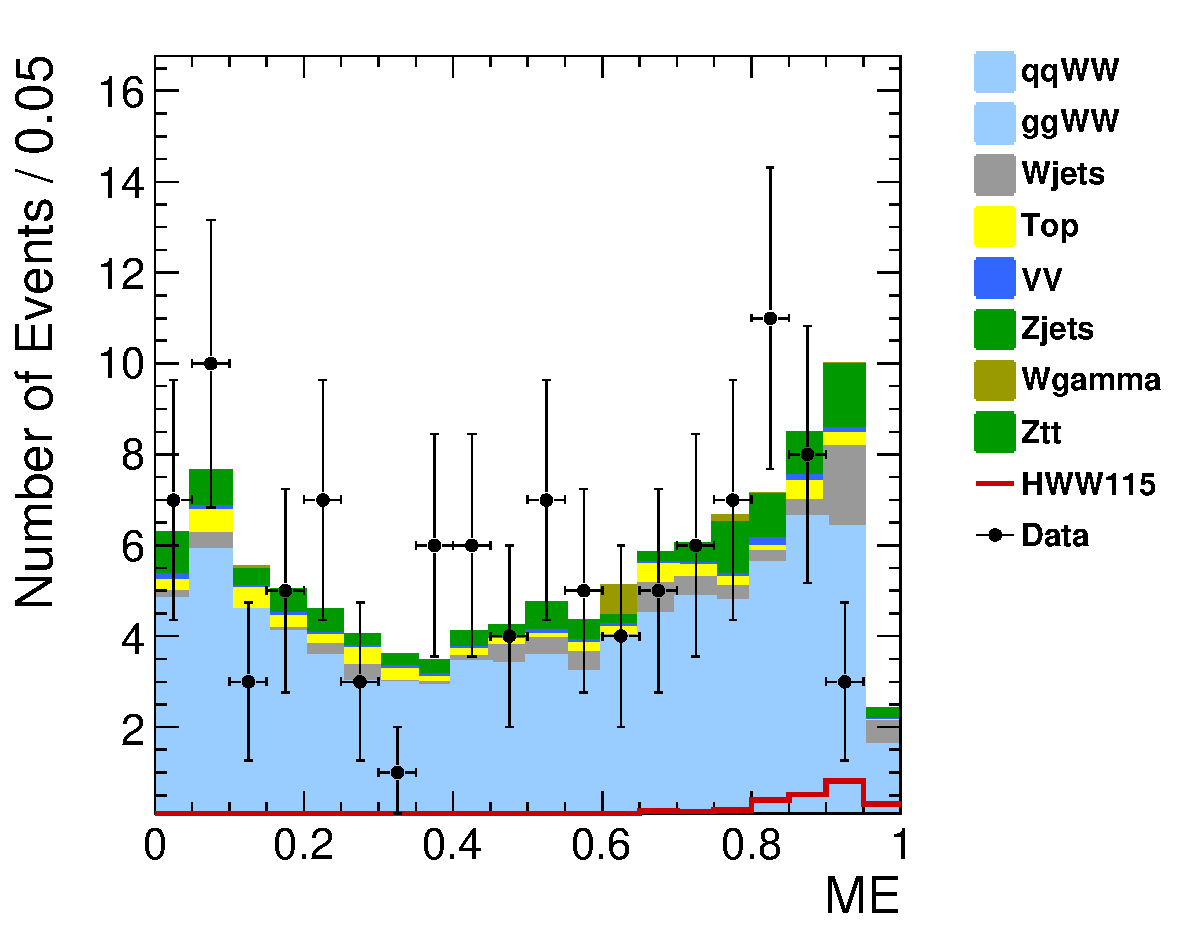
\includegraphics[width=.40\textwidth]{figures/ME_mH115_0j_sf_stack_lin.pdf}}
\subfigure[$e\mu$ 1-Jet]{
\centering
\label{subfig:me_115_1j_of_4700pb}
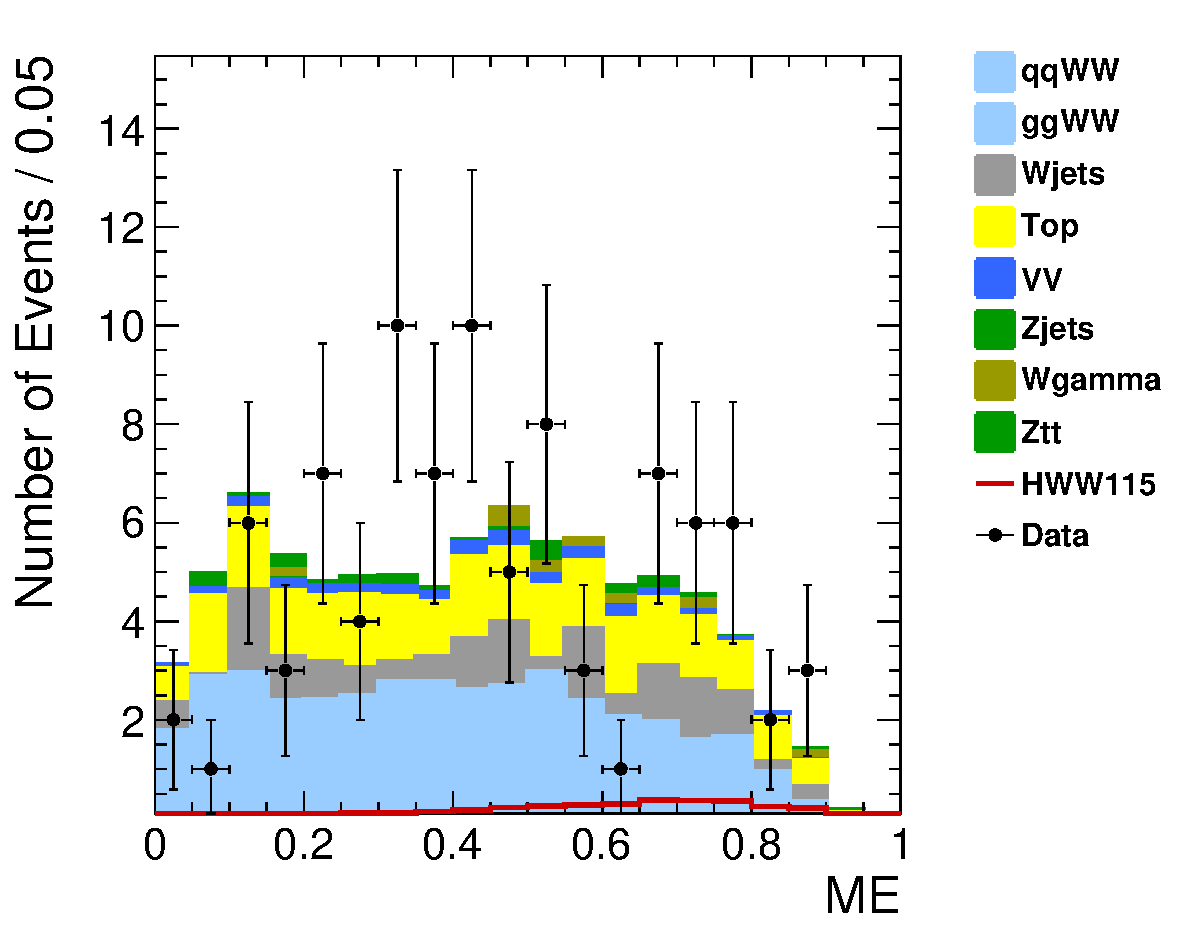
\includegraphics[width=.40\textwidth]{figures/ME_mH115_1j_of_stack_lin.pdf}}
\subfigure[$ee$/$\mu\mu$ 1-Jet]{
\centering
\label{subfig:me_115_1j_sf_4700pb}
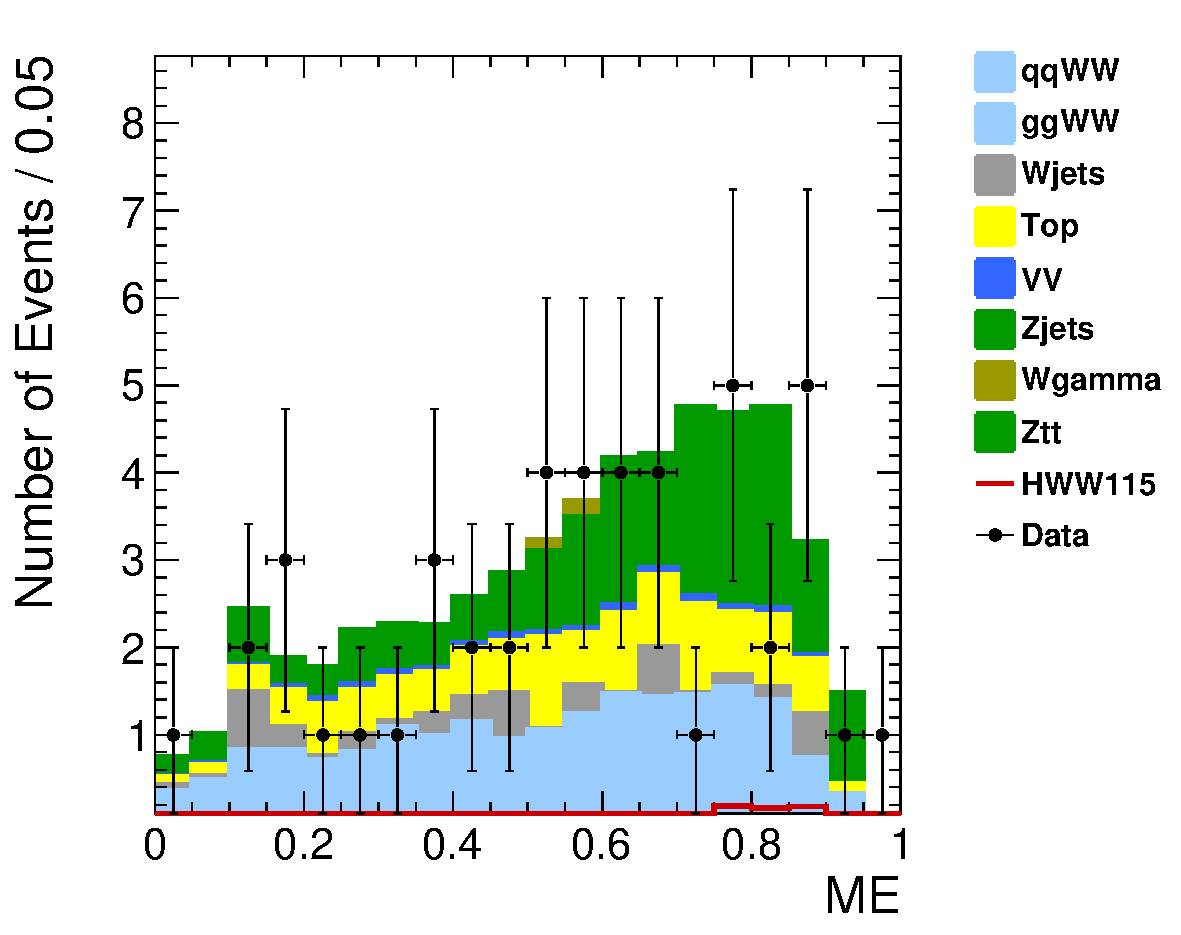
\includegraphics[width=.40\textwidth]{figures/ME_mH115_1j_sf_stack_lin.pdf}}
\caption{
ME output for $m_H$=115 GeV corresponding to \intlumi:
0-jet OF \subref{subfig:me_115_0j_of_4700pb},
0-jet SF \subref{subfig:me_115_0j_sf_4700pb},
1-jet OF \subref{subfig:me_115_1j_of_4700pb},
1-jet SF \subref{subfig:me_115_1j_sf_4700pb}
.}
\label{fig:me_115_4700pb}
\end{figure}

\begin{figure}[!hbtp]
\centering
\subfigure[$e\mu$ 0-Jet]{
\centering
\label{subfig:me_120_0j_of_4700pb}
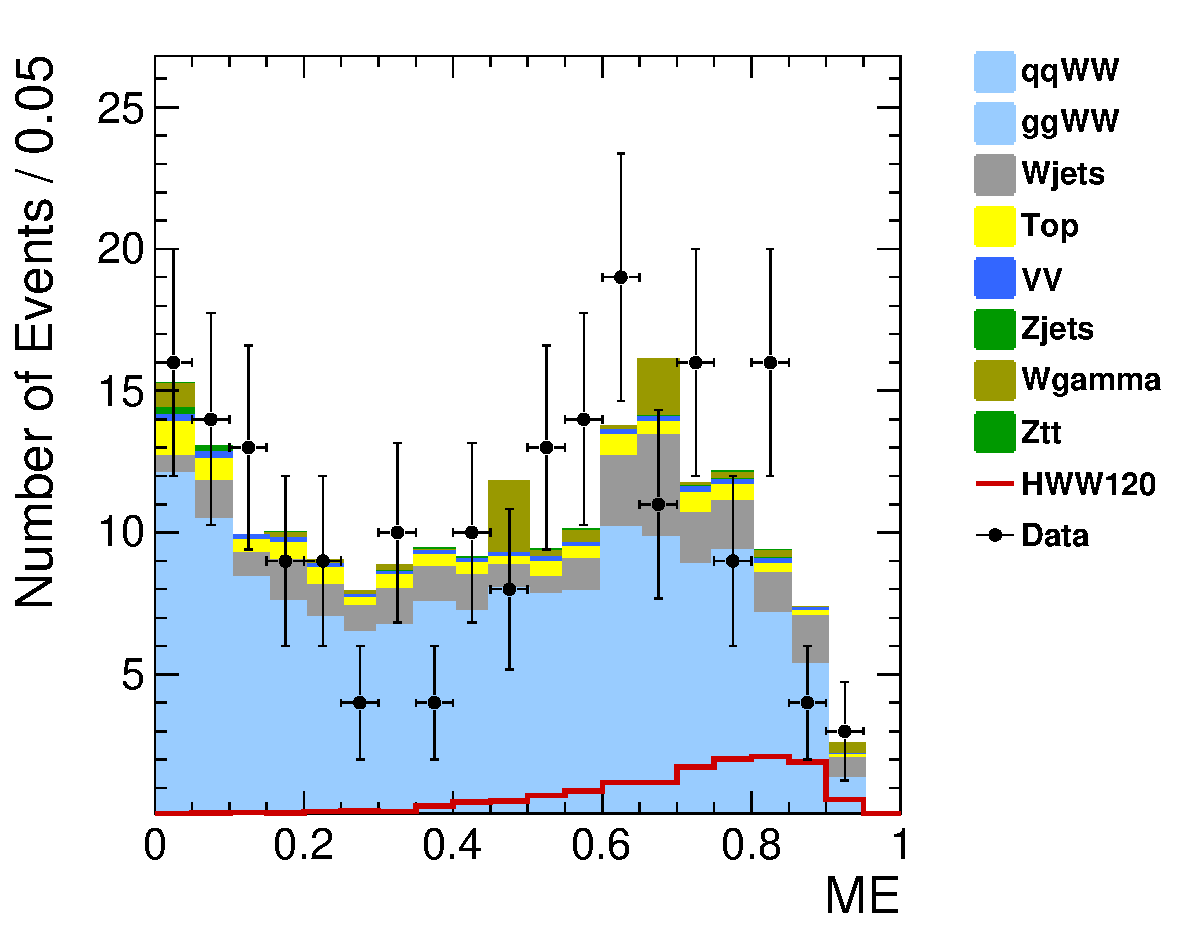
\includegraphics[width=.40\textwidth]{figures/ME_mH120_0j_of_stack_lin.pdf}}
\subfigure[$ee/\mu\mu$ 0-Jet]{
\centering
\label{subfig:me_120_0j_sf_4700pb}
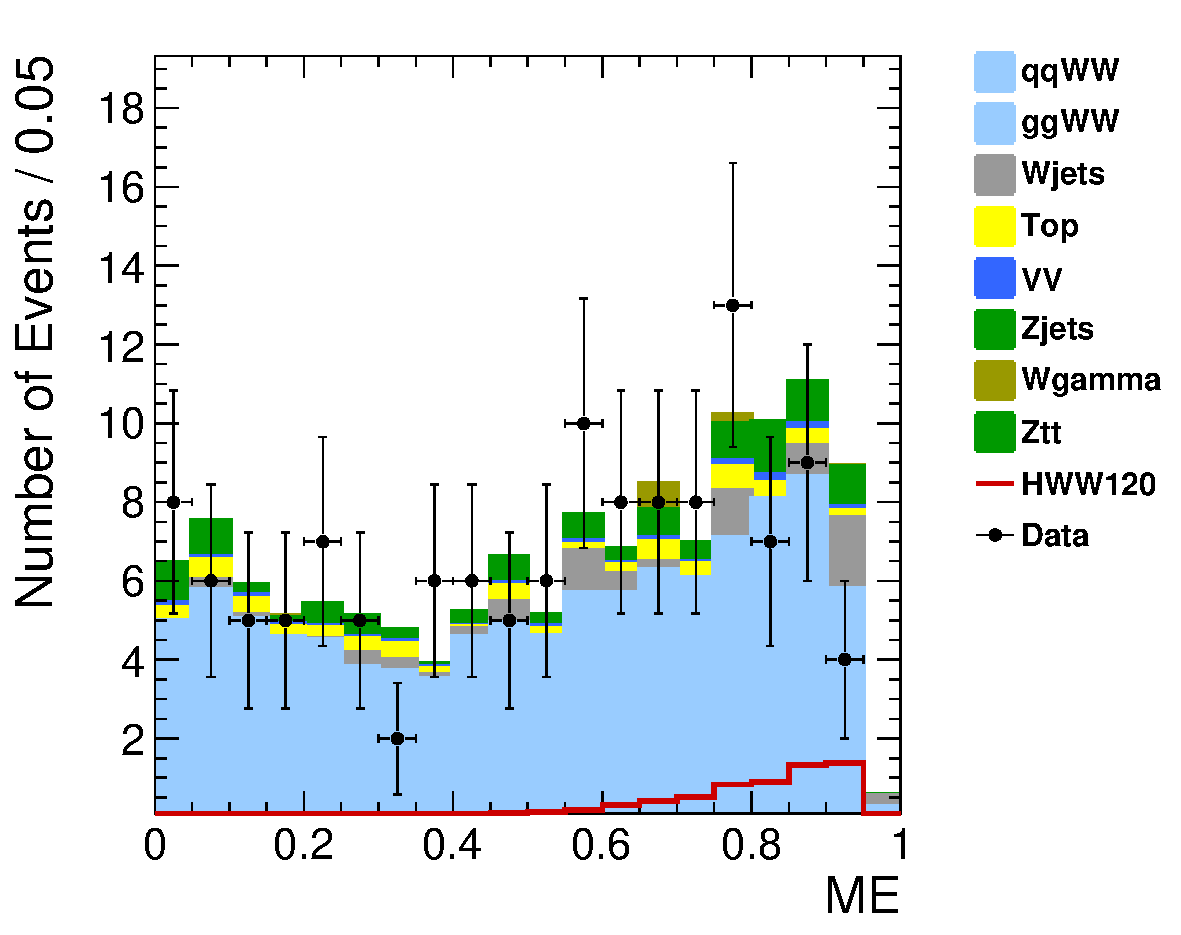
\includegraphics[width=.40\textwidth]{figures/ME_mH120_0j_sf_stack_lin.pdf}}
\subfigure[$e\mu$ 1-Jet]{
\centering
\label{subfig:me_120_1j_of_4700pb}
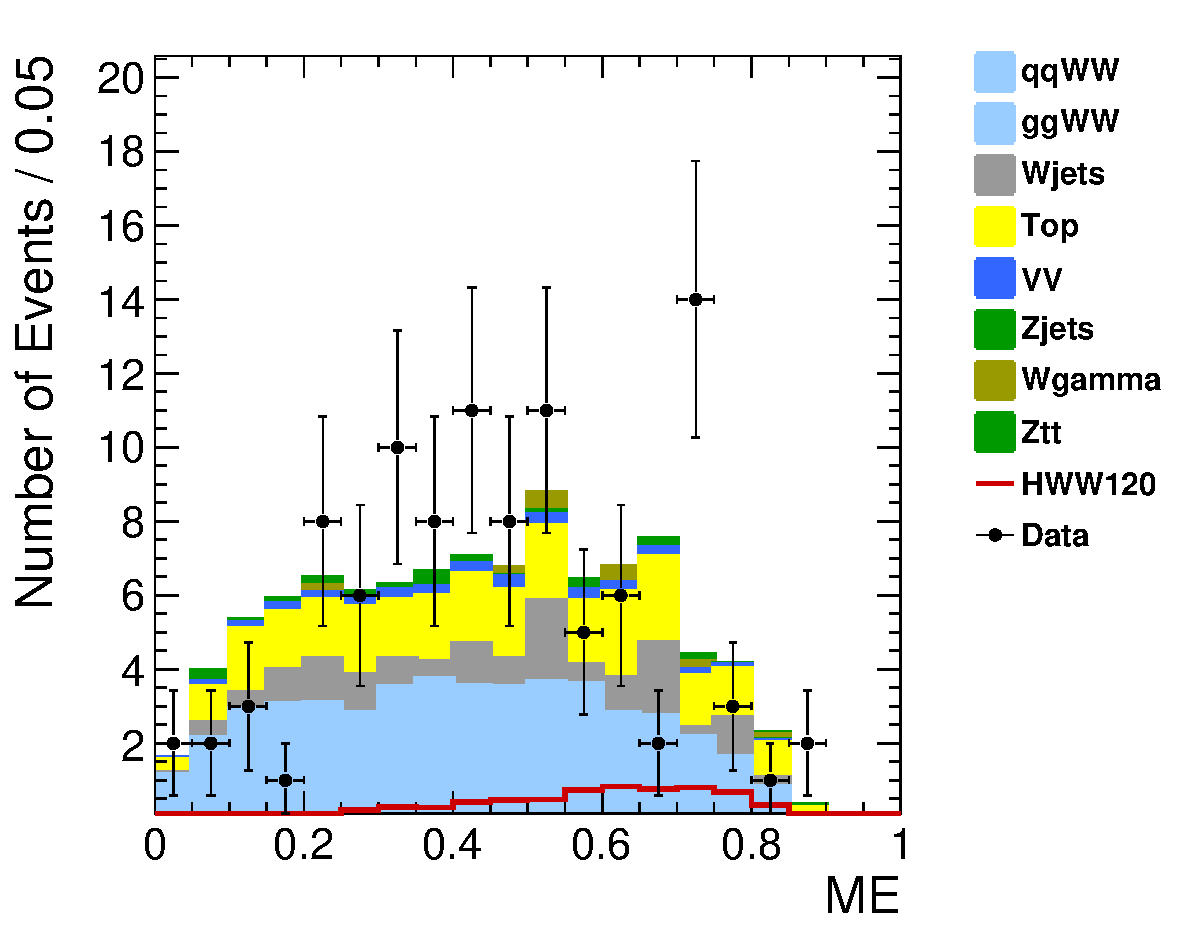
\includegraphics[width=.40\textwidth]{figures/ME_mH120_1j_of_stack_lin.pdf}}
\subfigure[$ee/\mu\mu$ 1-Jet]{
\centering
\label{subfig:me_120_1j_sf_4700pb}
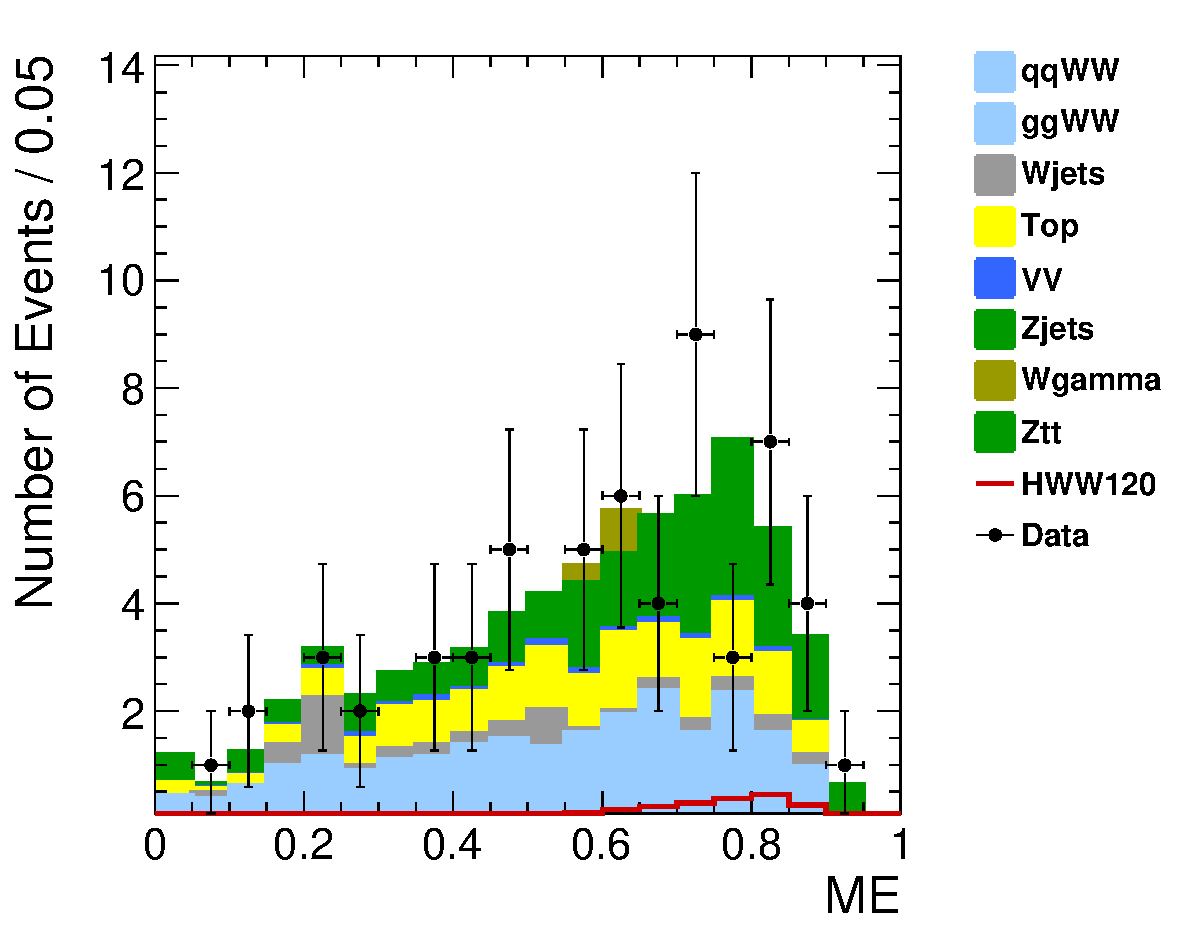
\includegraphics[width=.40\textwidth]{figures/ME_mH120_1j_sf_stack_lin.pdf}}
\caption{
ME output for $m_H$=120 GeV corresponding to \intlumi:
0-jet OF \subref{subfig:me_120_0j_of_4700pb},
0-jet SF \subref{subfig:me_120_0j_sf_4700pb},
1-jet OF \subref{subfig:me_120_1j_of_4700pb},
1-jet SF \subref{subfig:me_120_1j_sf_4700pb}.}
\label{fig:me_120_4700pb}
\end{figure}
%%%%%%%%%%%%%%%%%%%%%%%%%%%%%%%%%%%%%

%%%%%%%%%%%%%%%%%%%%%%%%%%%%%%%%%%%%%
\begin{figure}[!hbtp]
\centering
\subfigure[$e\mu$ 0-Jet]{
\centering
\label{subfig:me_130_0j_of_4700pb}
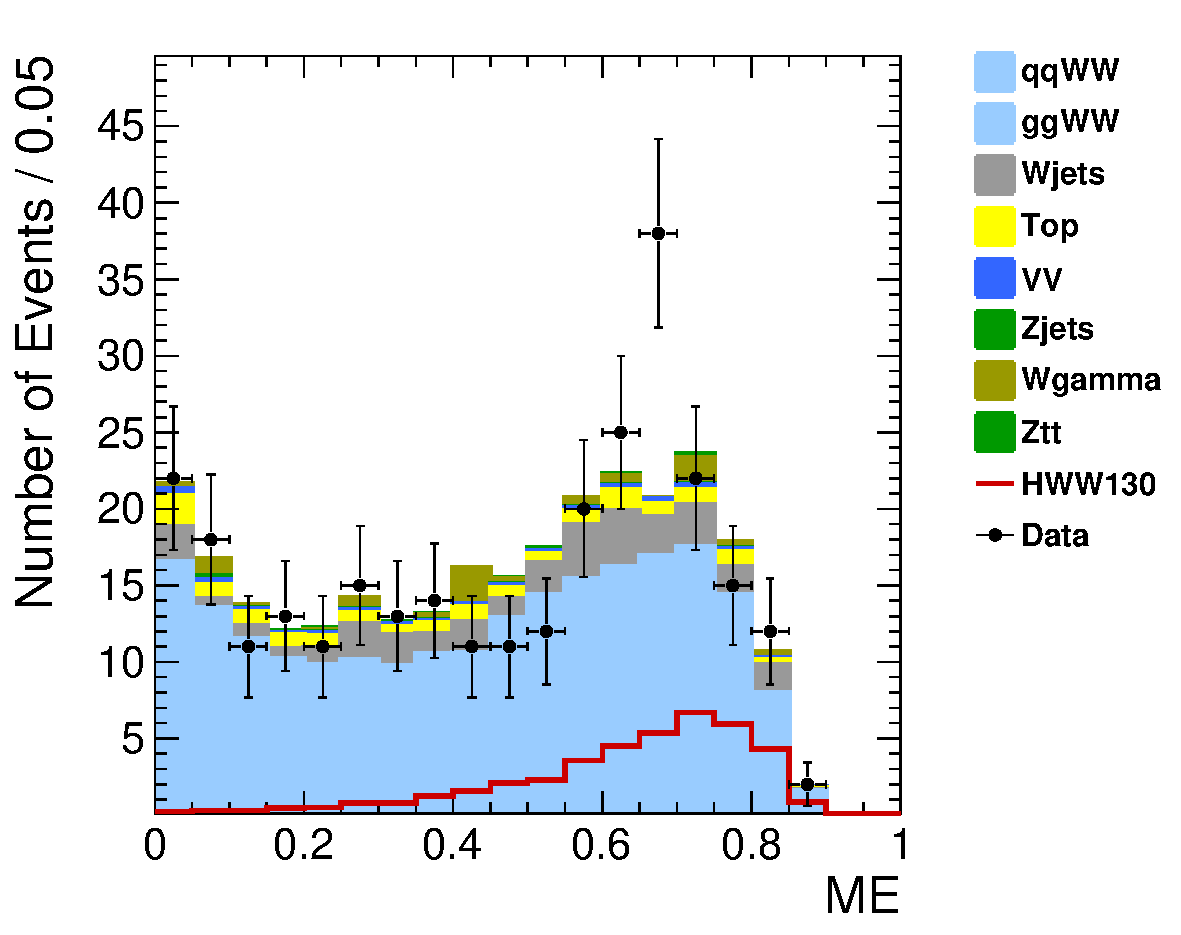
\includegraphics[width=.40\textwidth]{figures/ME_mH130_0j_of_stack_lin.pdf}}
\subfigure[$ee/\mu\mu$ 0-Jet]{
\centering
\label{subfig:me_130_0j_sf_4700pb}
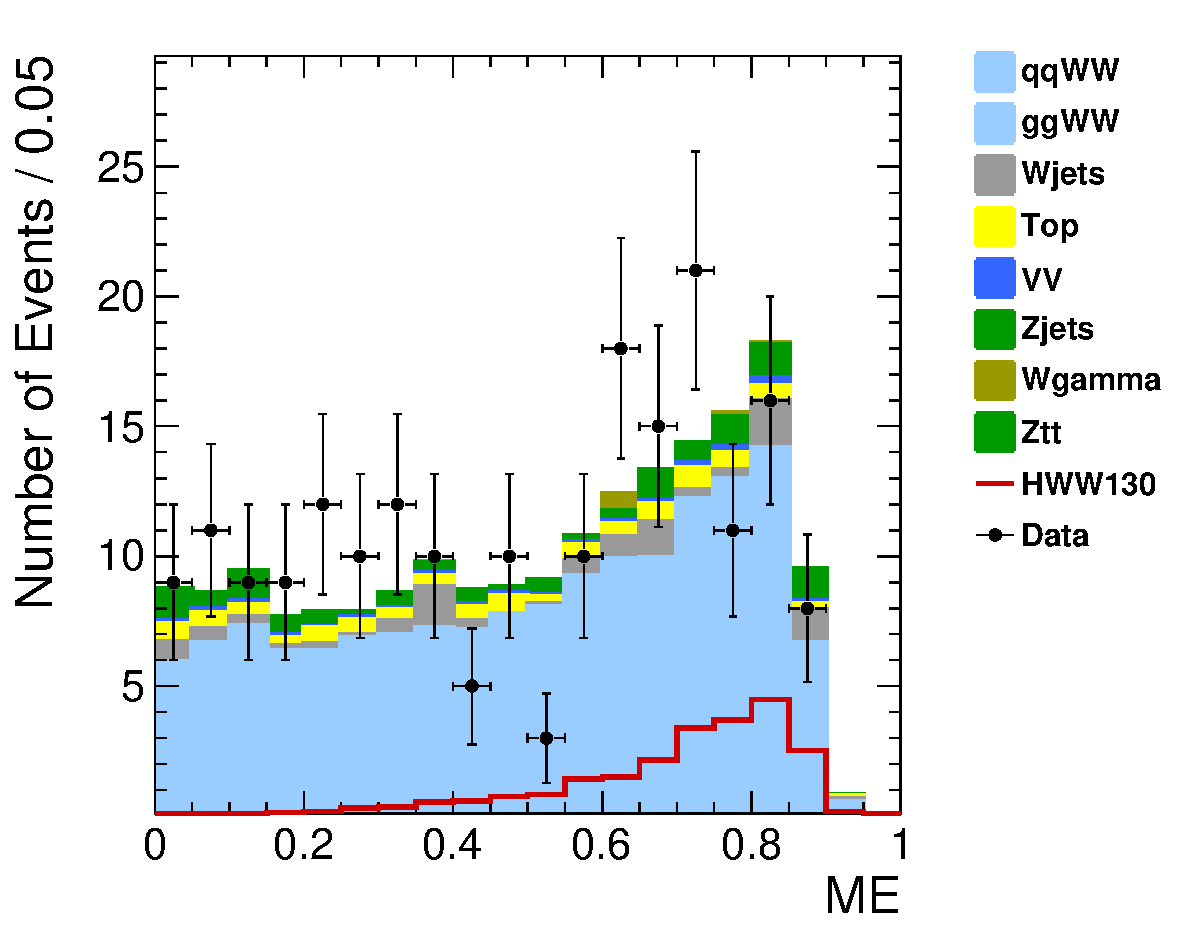
\includegraphics[width=.40\textwidth]{figures/ME_mH130_0j_sf_stack_lin.pdf}}
\subfigure[$e\mu$ 1-Jet]{
\centering
\label{subfig:me_130_1j_of_4700pb}
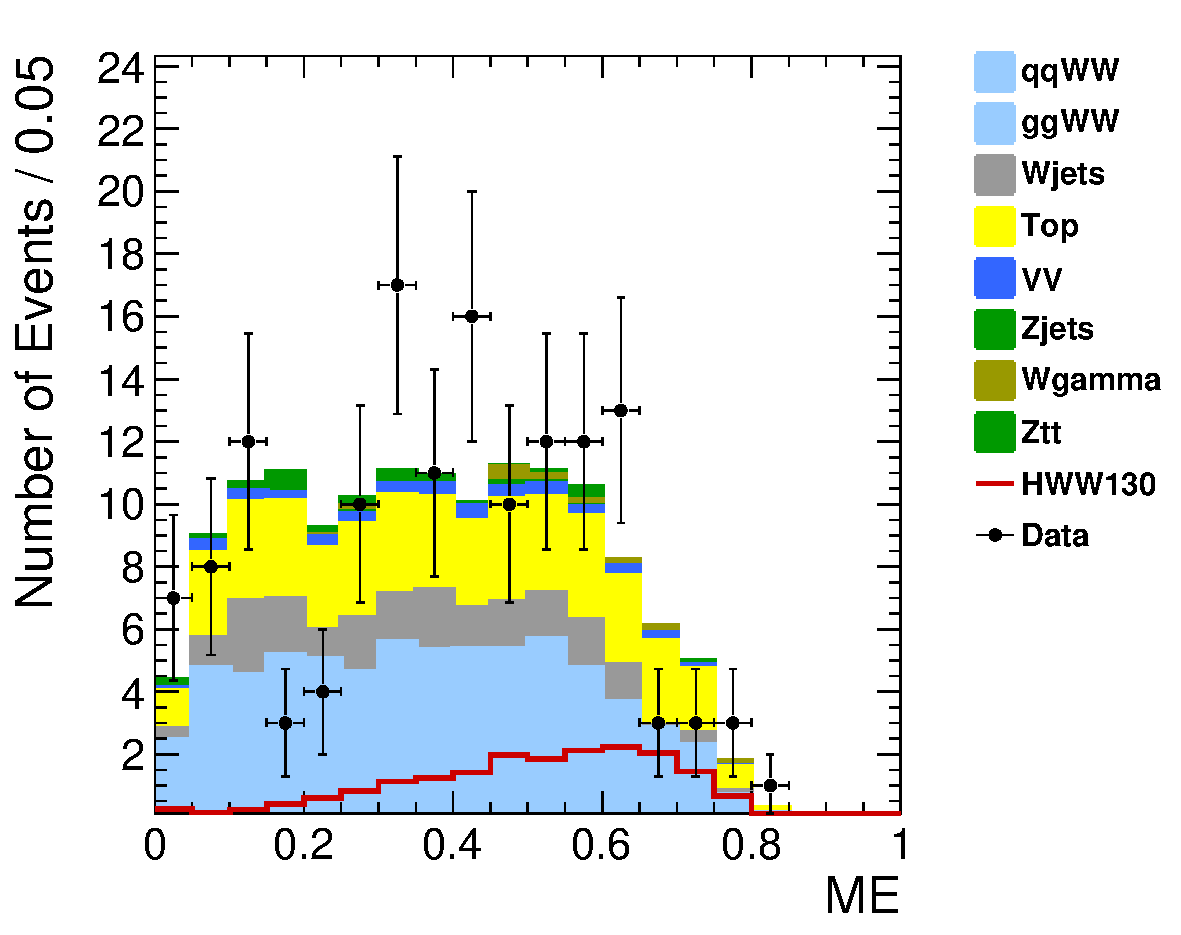
\includegraphics[width=.40\textwidth]{figures/ME_mH130_1j_of_stack_lin.pdf}}
\subfigure[$ee/\mu\mu$ 1-Jet]{
\centering
\label{subfig:me_130_1j_sf_4700pb}
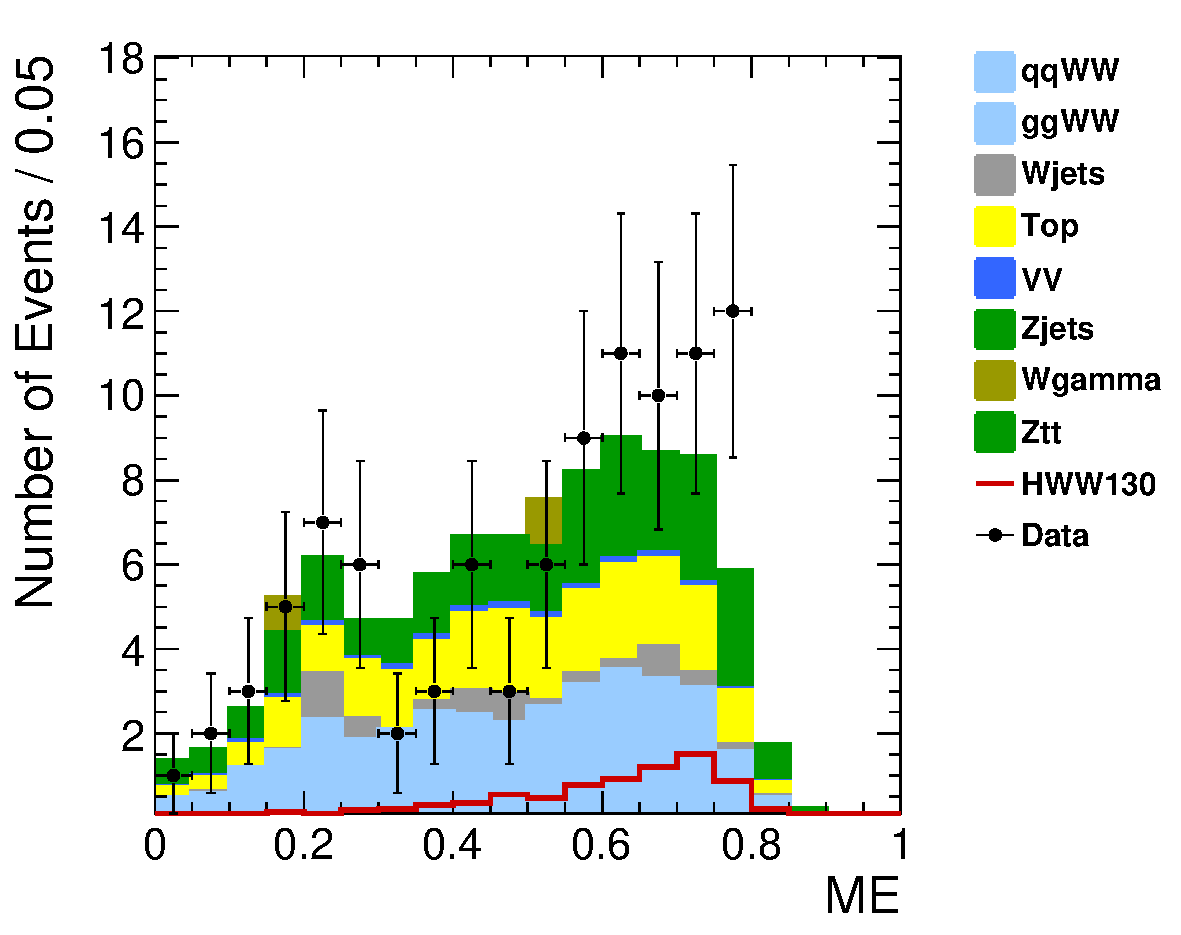
\includegraphics[width=.40\textwidth]{figures/ME_mH130_1j_sf_stack_lin.pdf}}
\caption{
ME output for $m_H$=130 GeV corresponding to \intlumi:
0-jet OF \subref{subfig:me_130_0j_of_4700pb},
0-jet SF \subref{subfig:me_130_0j_sf_4700pb},
1-jet OF \subref{subfig:me_130_1j_of_4700pb},
1-jet SF \subref{subfig:me_130_1j_sf_4700pb}
.}
\label{fig:me_130_4700pb}
\end{figure}
%%%%%%%%%%%%%%%%%%%%%%%%%%%%%%%%%%%%%

%%%%%%%%%%%%%%%%%%%%%%%%%%%%%%%%%%%%%
\begin{figure}[!hbtp]
\centering
\subfigure[$e\mu$ 0-Jet]{
\centering
\label{subfig:me_140_0j_of_4700pb}
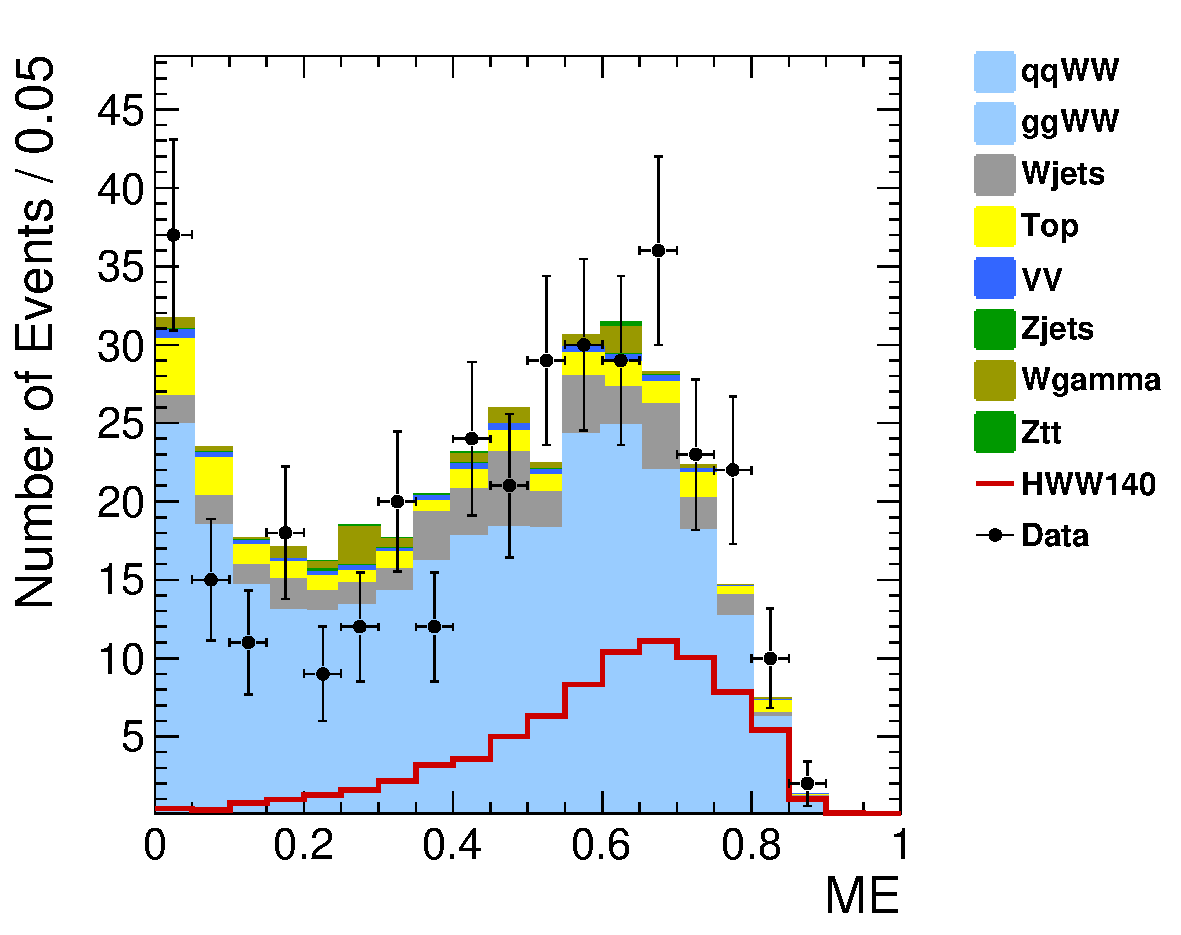
\includegraphics[width=.40\textwidth]{figures/ME_mH140_0j_of_stack_lin.pdf}}
\subfigure[$ee/\mu\mu$ 0-Jet]{
\centering
\label{subfig:me_140_0j_sf_4700pb}
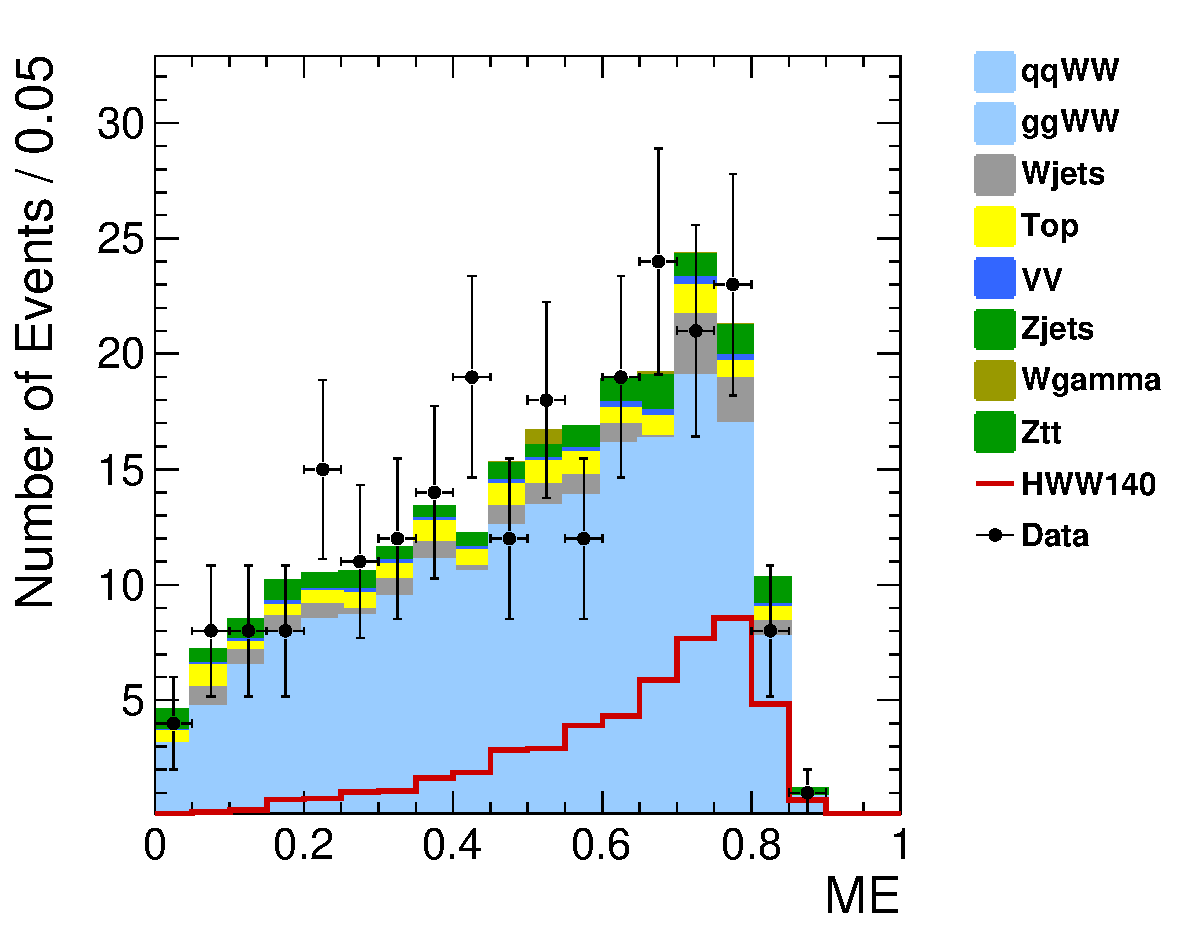
\includegraphics[width=.40\textwidth]{figures/ME_mH140_0j_sf_stack_lin.pdf}}
\subfigure[$e\mu$ 1-Jet]{
\centering
\label{subfig:me_140_1j_of_4700pb}
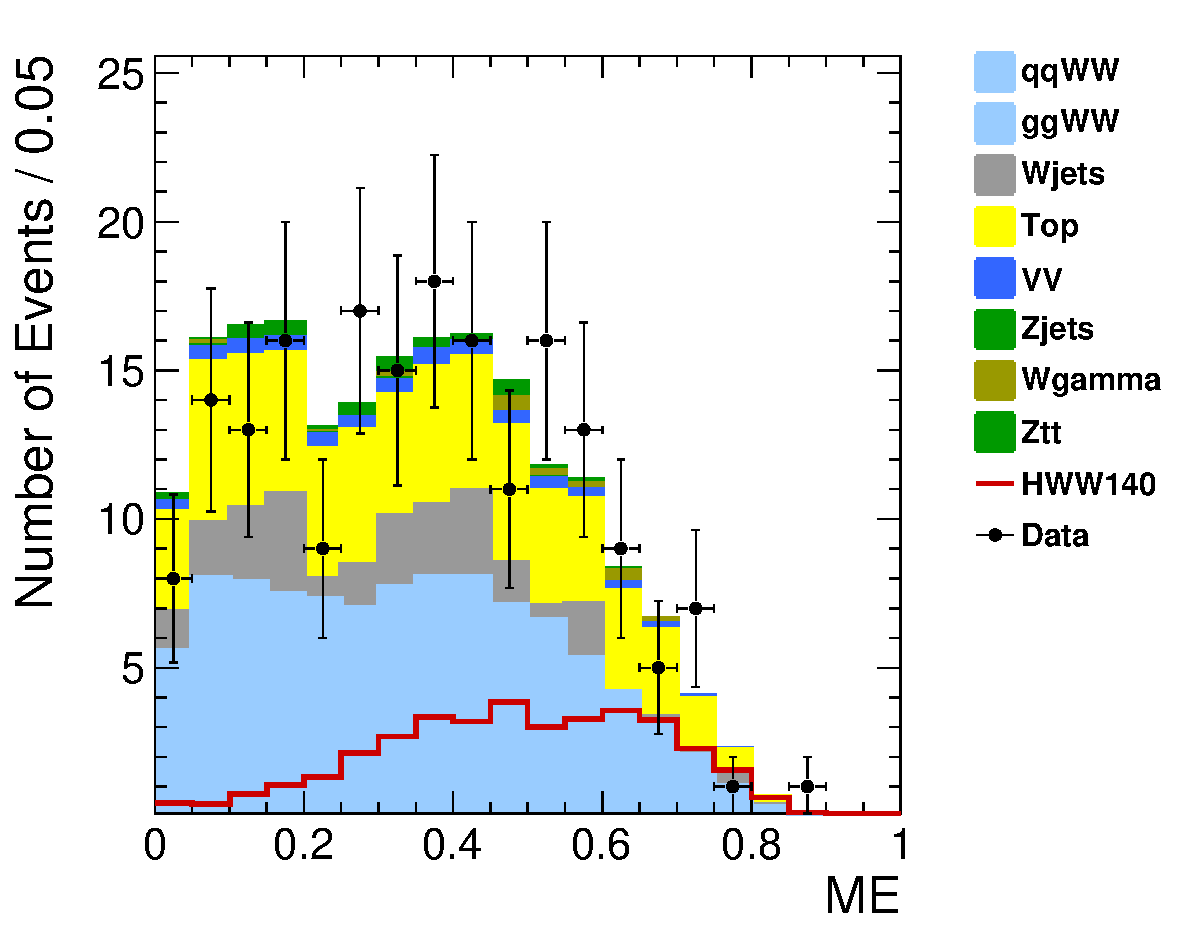
\includegraphics[width=.40\textwidth]{figures/ME_mH140_1j_of_stack_lin.pdf}}
\subfigure[$ee/\mu\mu$ 1-Jet]{
\centering
\label{subfig:me_140_1j_sf_4700pb}
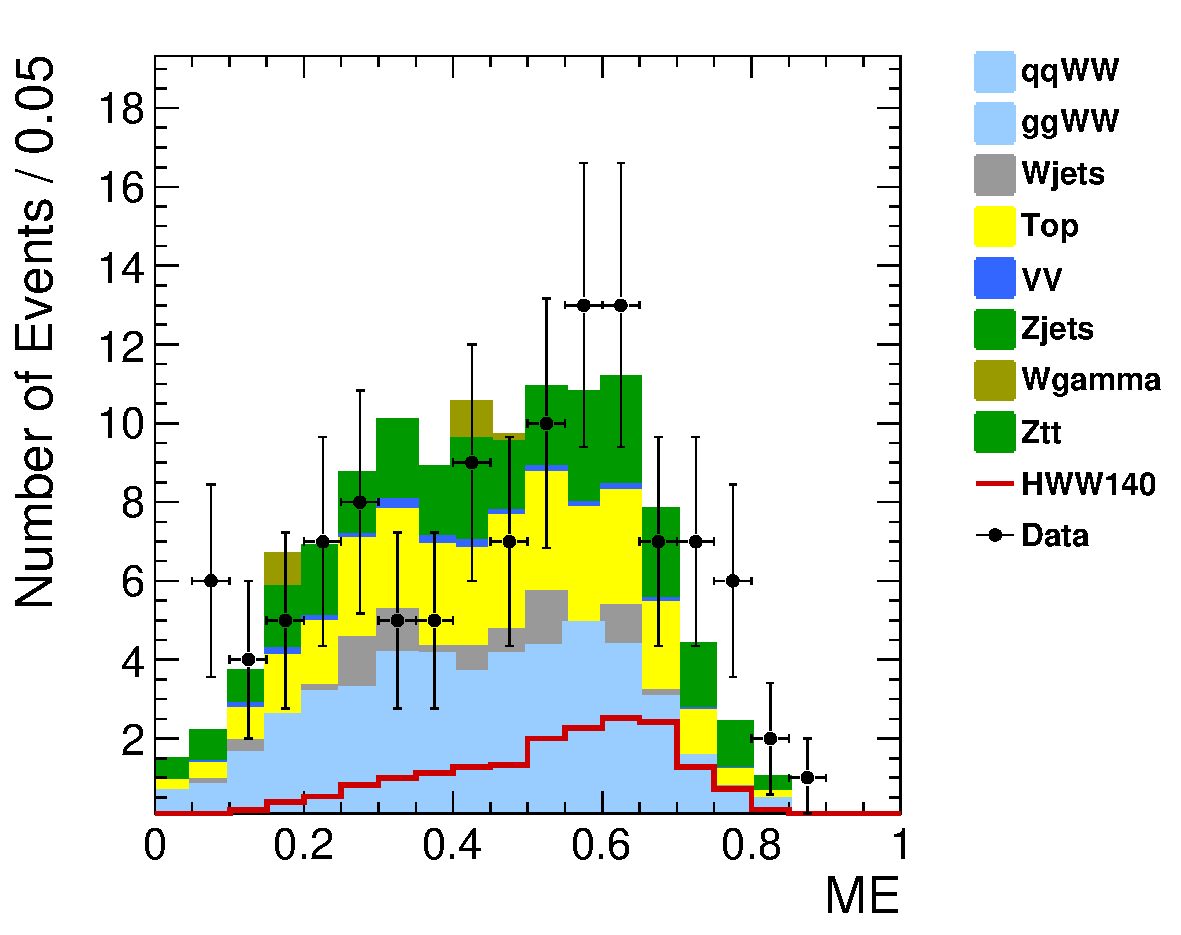
\includegraphics[width=.40\textwidth]{figures/ME_mH140_1j_sf_stack_lin.pdf}}
\caption{
ME output for $m_H$=140 GeV corresponding to \intlumi:
0-jet OF \subref{subfig:me_140_0j_of_4700pb},
0-jet SF \subref{subfig:me_140_0j_sf_4700pb},
1-jet OF \subref{subfig:me_140_1j_of_4700pb},
1-jet SF \subref{subfig:me_140_1j_sf_4700pb}
.}
\label{fig:me_140_4700pb}
\end{figure}
%%%%%%%%%%%%%%%%%%%%%%%%%%%%%%%%%%%%%


              
%%%%%%%%%%%%%%%%%%%%%%%%%%%%%%%%%%%%%
\begin{figure}[!hbtp]
\centering
\subfigure[$e\mu$ 0-Jet]{
\centering
\label{subfig:me_160_0j_of_4700pb}
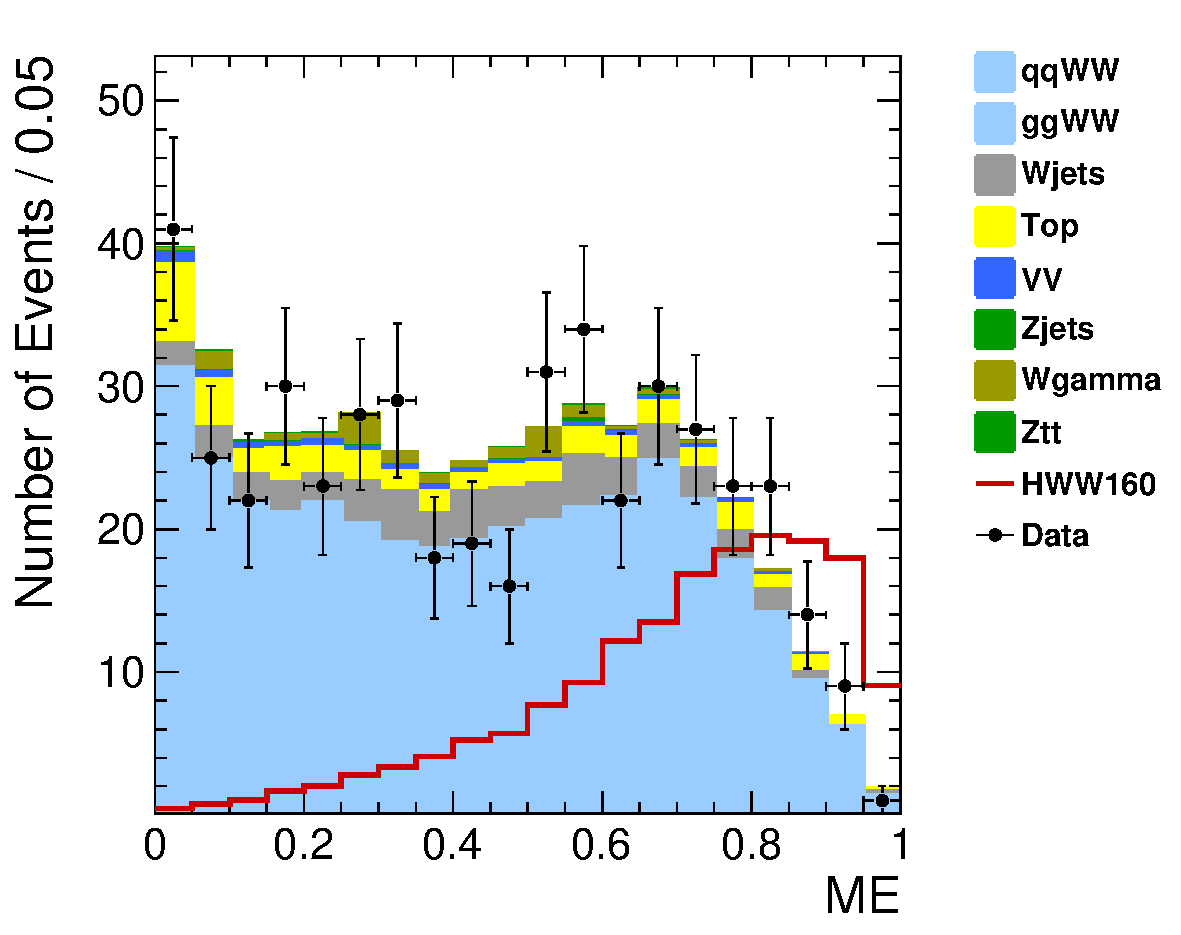
\includegraphics[width=.40\textwidth]{figures/ME_mH160_0j_of_stack_lin.pdf}}
\subfigure[$ee/\mu\mu$ 0-Jet]{
\centering
\label{subfig:me_160_0j_sf_4700pb}
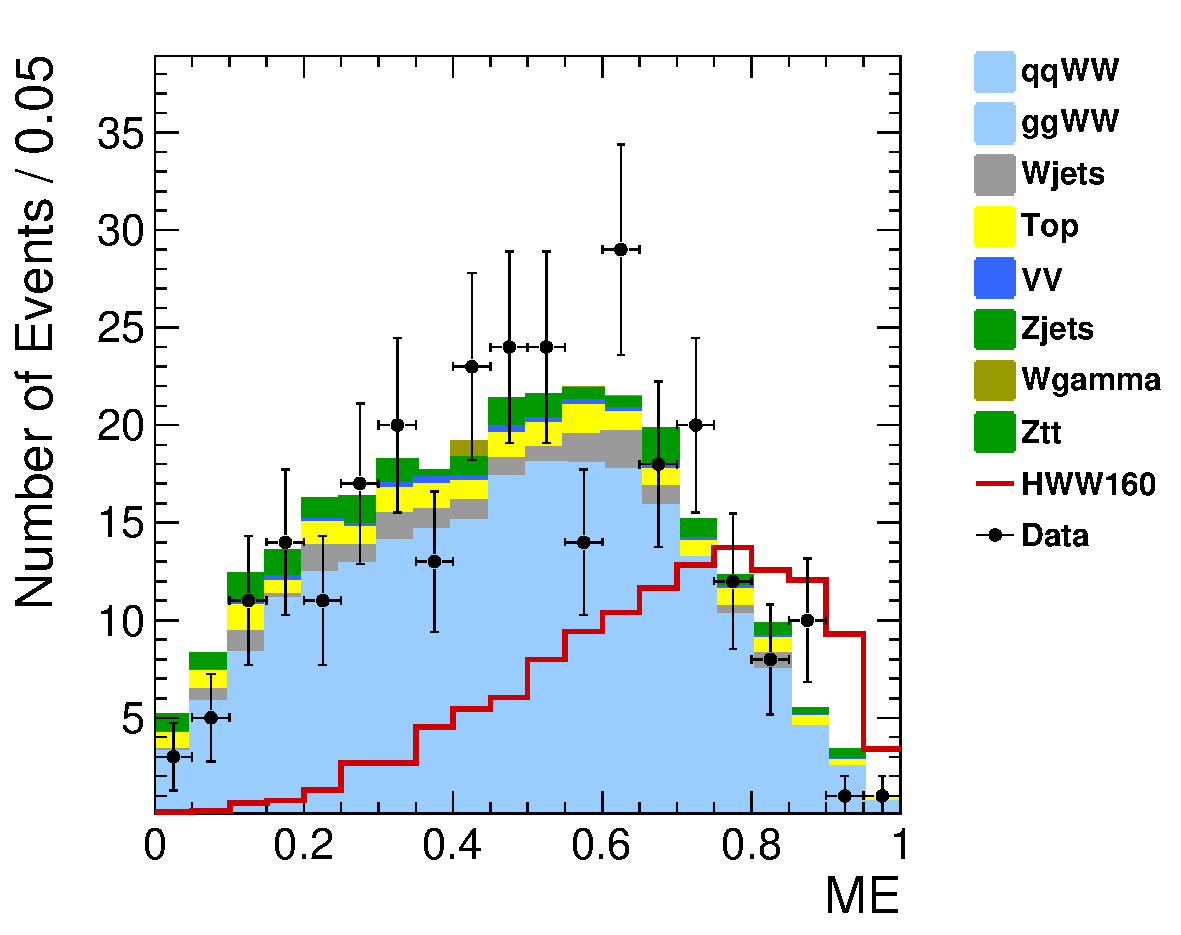
\includegraphics[width=.40\textwidth]{figures/ME_mH160_0j_sf_stack_lin.pdf}}
\subfigure[$e\mu$ 1-Jet]{
\centering
\label{subfig:me_160_1j_of_4700pb}
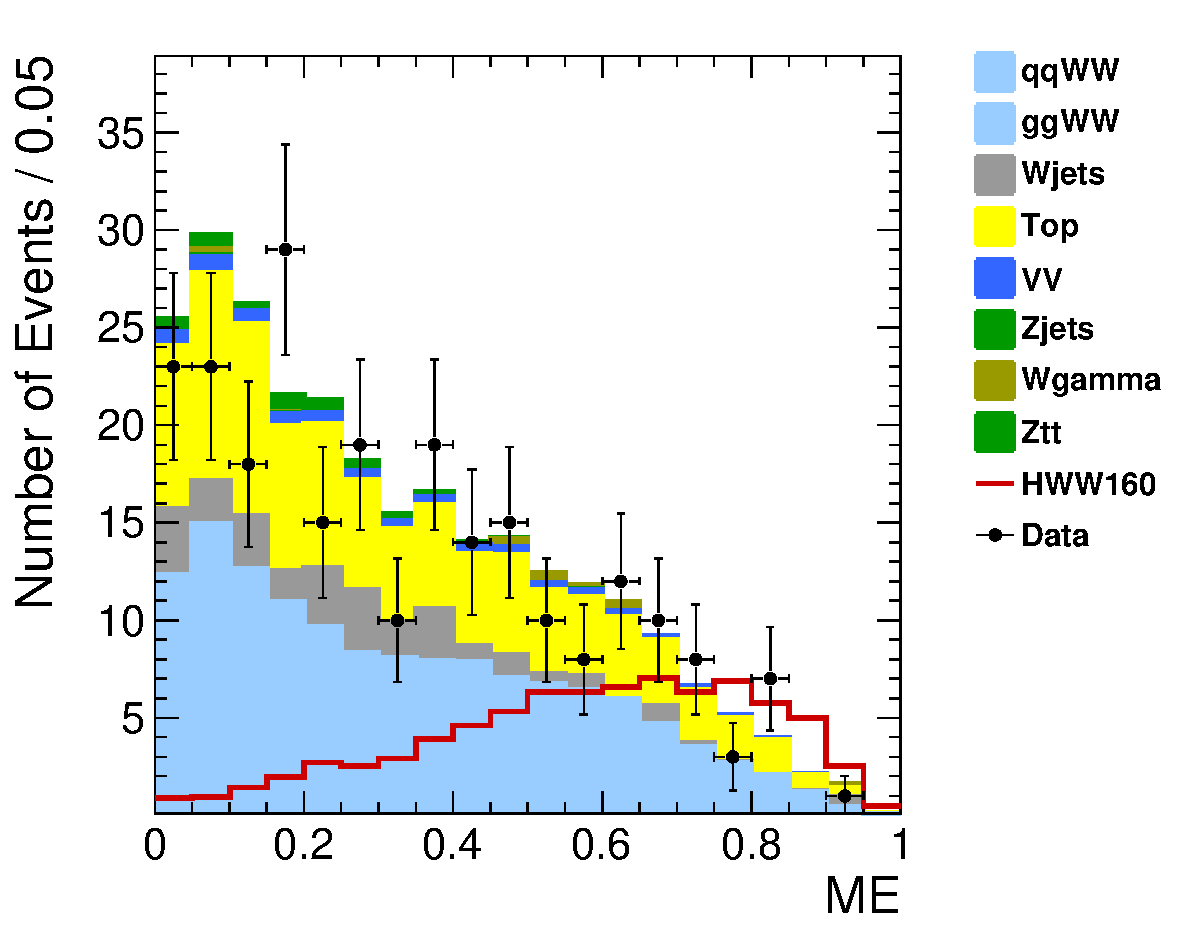
\includegraphics[width=.40\textwidth]{figures/ME_mH160_1j_of_stack_lin.pdf}}
\subfigure[$ee/\mu\mu$ 1-Jet]{
\centering
\label{subfig:me_160_1j_sf_4700pb}
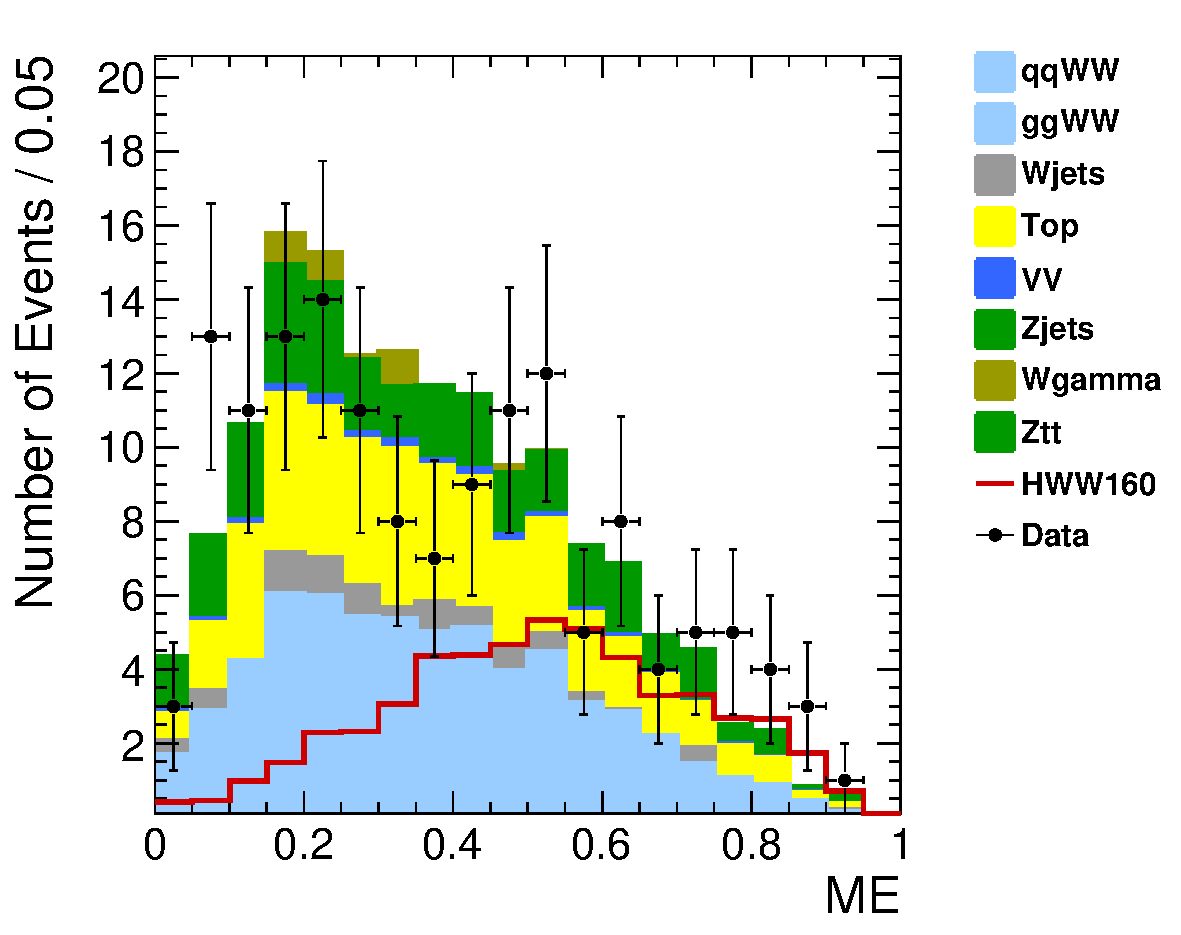
\includegraphics[width=.40\textwidth]{figures/ME_mH160_1j_sf_stack_lin.pdf}}
\caption{
ME output for $m_H$=160 GeV corresponding to \intlumi:
0-jet OF \subref{subfig:me_160_0j_of_4700pb},
0-jet SF \subref{subfig:me_160_0j_sf_4700pb},
1-jet OF \subref{subfig:me_160_1j_of_4700pb},
1-jet SF \subref{subfig:me_160_1j_sf_4700pb}
.}
\label{fig:me_160_4700pb}
\end{figure}
%%%%%%%%%%%%%%%%%%%%%%%%%%%%%%%%%%%%%
  

              
%%%%%%%%%%%%%%%%%%%%%%%%%%%%%%%%%%%%%
\begin{figure}[!hbtp]
\centering
\subfigure[$e\mu$ 0-Jet]{
\centering
\label{subfig:me_200_0j_of_4700pb}
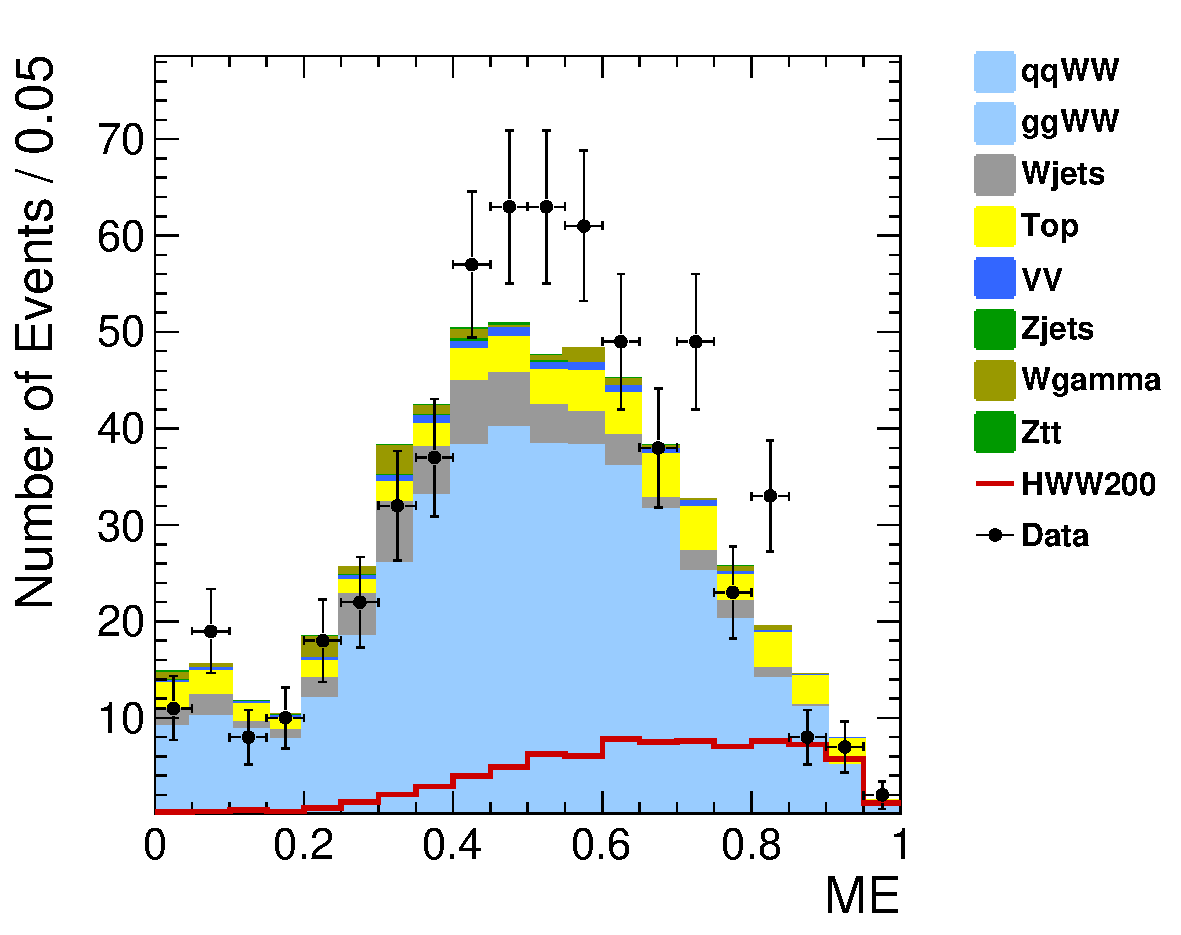
\includegraphics[width=.40\textwidth]{figures/ME_mH200_0j_of_stack_lin.pdf}}
\subfigure[$ee/\mu\mu$ 0-Jet]{
\centering
\label{subfig:me_200_0j_sf_4700pb}
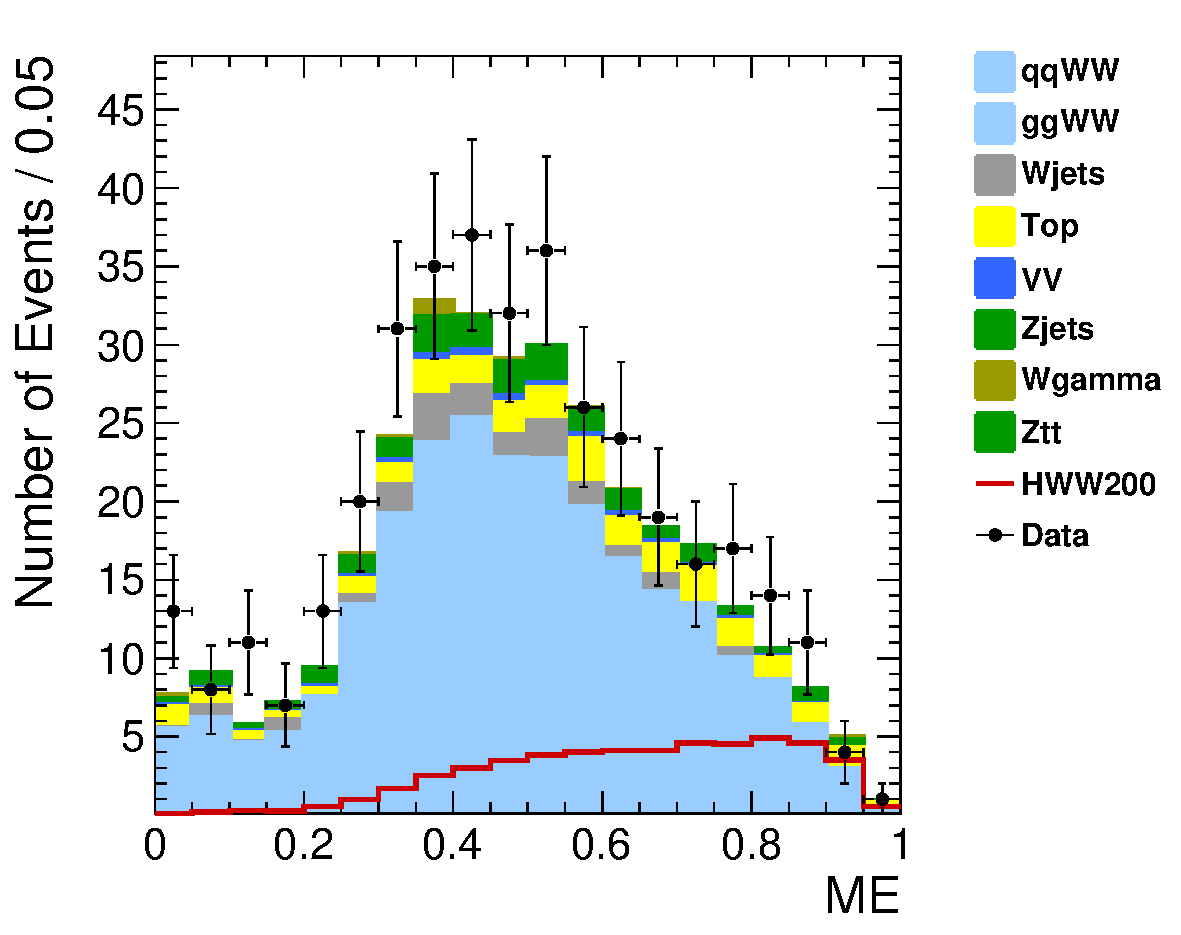
\includegraphics[width=.40\textwidth]{figures/ME_mH200_0j_sf_stack_lin.pdf}}
\subfigure[$e\mu$ 1-Jet]{
\centering
\label{subfig:me_200_1j_of_4700pb}
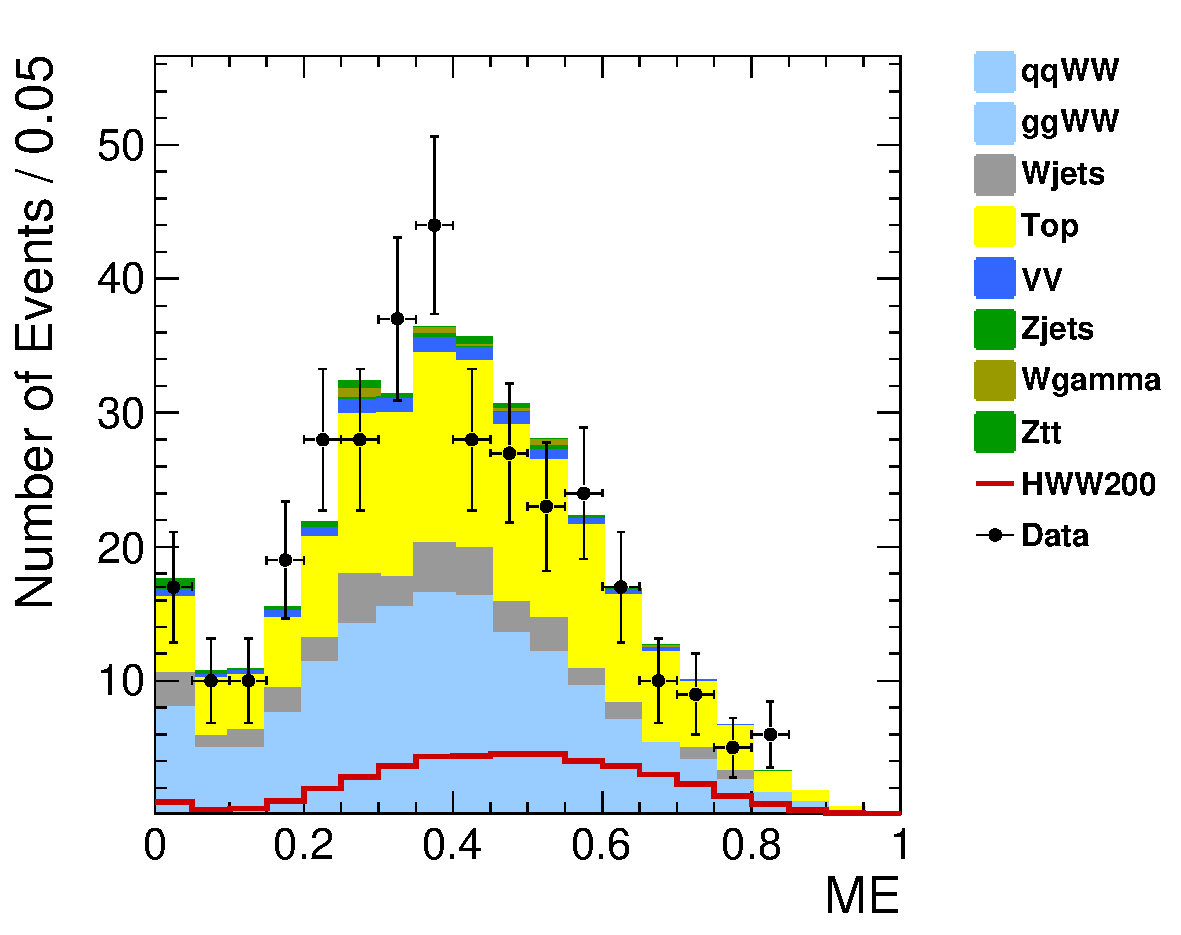
\includegraphics[width=.40\textwidth]{figures/ME_mH200_1j_of_stack_lin.pdf}}
\subfigure[$ee/\mu\mu$ 1-Jet]{
\centering
\label{subfig:me_200_1j_sf_4700pb}
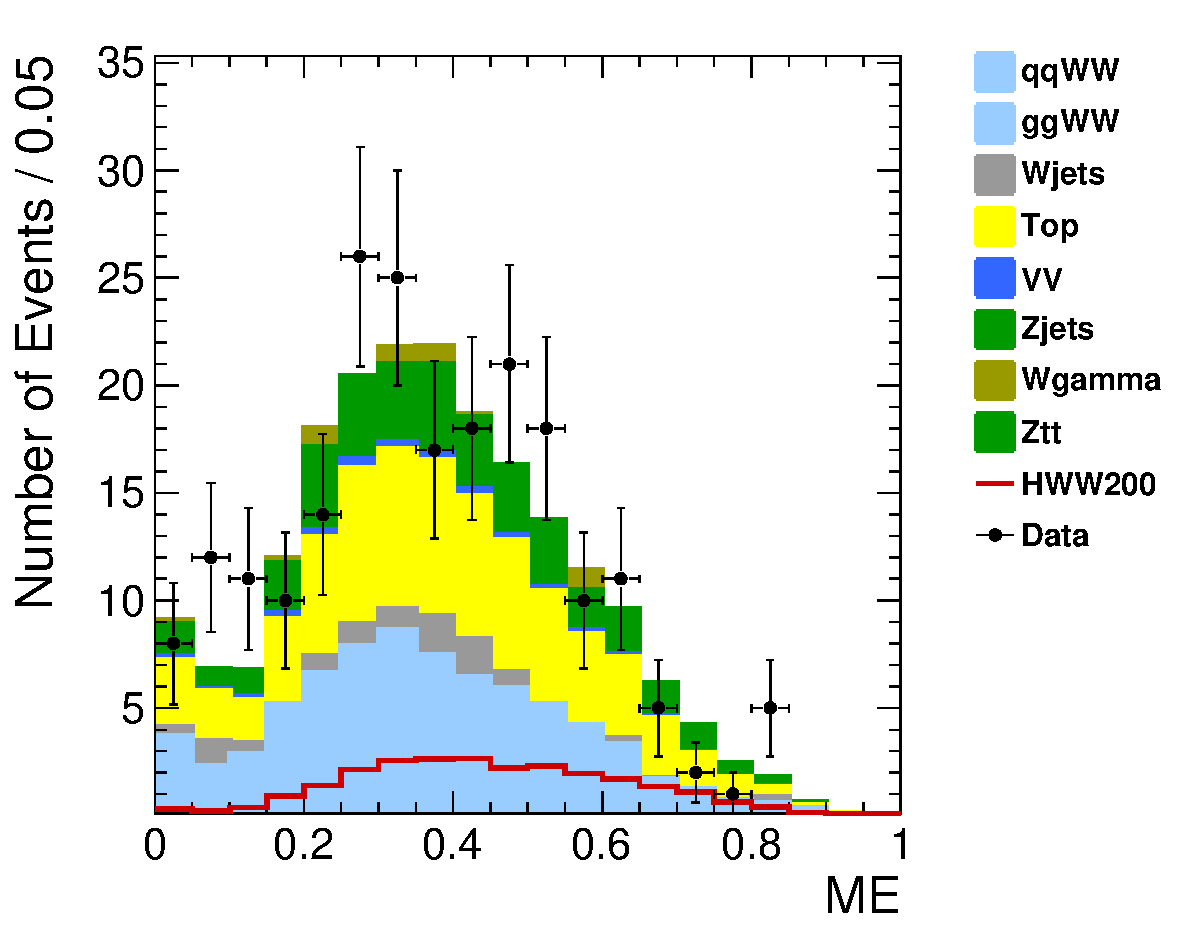
\includegraphics[width=.40\textwidth]{figures/ME_mH200_1j_sf_stack_lin.pdf}}
\caption{
ME output for $m_H$=200 GeV corresponding to \intlumi:
0-jet OF \subref{subfig:me_200_0j_of_4700pb},
0-jet SF \subref{subfig:me_200_0j_sf_4700pb},
1-jet OF \subref{subfig:me_200_1j_of_4700pb},
1-jet SF \subref{subfig:me_200_1j_sf_4700pb}
.}
\label{fig:me_200_4700pb}
\end{figure}
%%%%%%%%%%%%%%%%%%%%%%%%%%%%%%%%%%%%%

Systematics uncertainties applied in the search are summarized in \cite{ref:HZZ2011smurf}.
Systematic variations affecting shapes of the likelihood ratio discriminant are included in the results presented in this note,
however methods to account for them are discussed separately in \cite{ref:ShapeSmurf}. 


The expected and observed upper limits at 95\%C.L., for the dataset corresponding to $\intlumi$ for 
the shape analysis based on the matrix element outputs are shown in Table~\ref{tab:me_results_5fb} and 
Figure~\ref{fig:me_results_5fb} for the 0/1/2 jet bins combined. 
The limits are obtained using the CLs asymptotic methods. 
The sensitivity performance of the matrix element method and the observed limits are 
consistent with the BDT-based approach. 

We also compare the performance for the 4 sub-channels individually, shown in 
Table~\ref{tab:me_results_5fb_0jsf}-\ref{tab:me_results_5fb_1jof} and Figure~\ref{fig:me_results_5fb_subchannel}. 
%Table~\ref{tab:me_results_5fb_0j}-\ref{tab:me_results_5fb_1j} show the comparison of the performance 
%in the 0 and 1 jet bins respectively. 

%To summarize, using matrix element based approach in $H\rightarrow WW \rightarrow l^{+}l^{-}\nu\bar{\nu}$ 
%we exclude Standard Model Higgs boson in the 128--X GeV mass range, with expected exclusion range of 128--X GeV at 95\% C.L. 
%For comparison, BDT expected and observed exclusion ranges in the 0-jet channel are similar: 128--X GeV and 128--X GeV, respectively.  


%%%%%%%%%%%%%%%%%%%%%%%%%%%%%%
\begin{figure}[!hbtp]
\centering
\subfigure[BDT]{
\centering
\label{subfig:bdt}
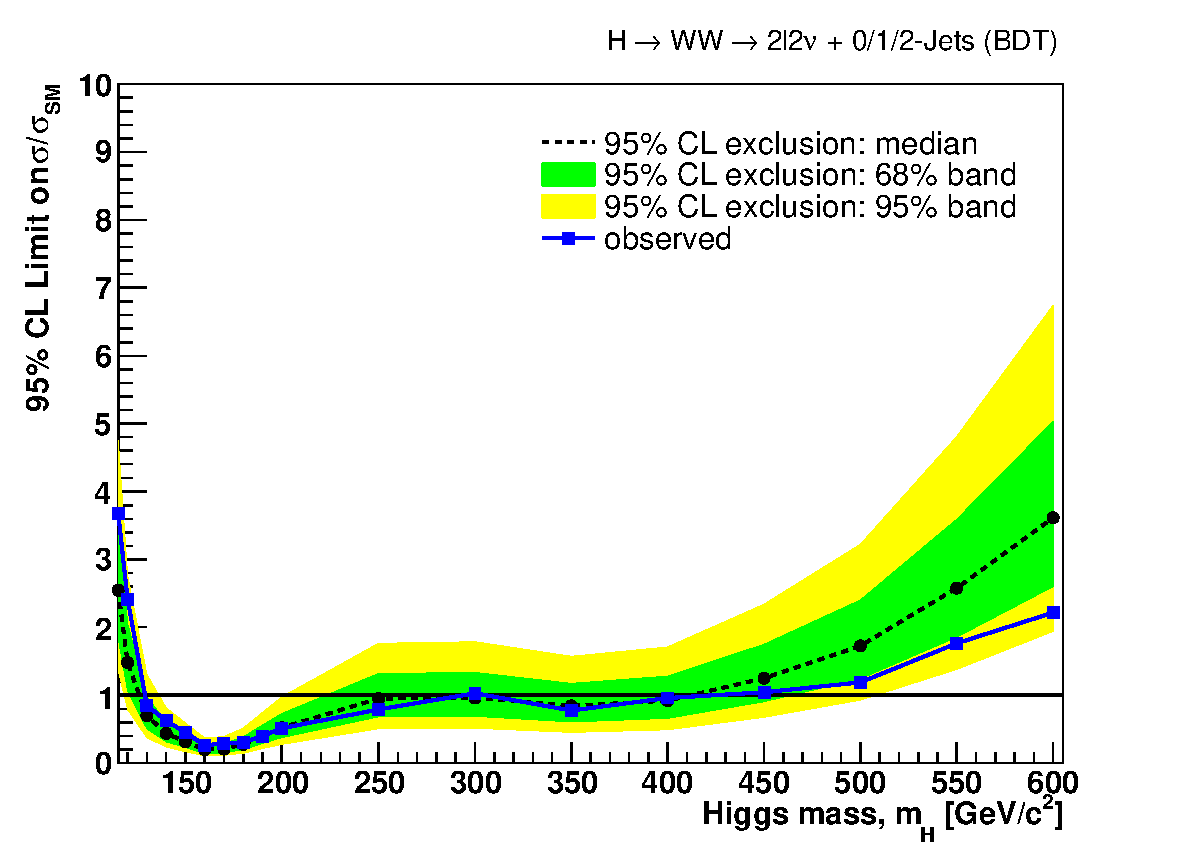
\includegraphics[width=.45\textwidth]{figures/limit_nj_shape_bdt-CLs-asymptotic.pdf}}
\subfigure[ME]{
\centering
\label{subfig:me}
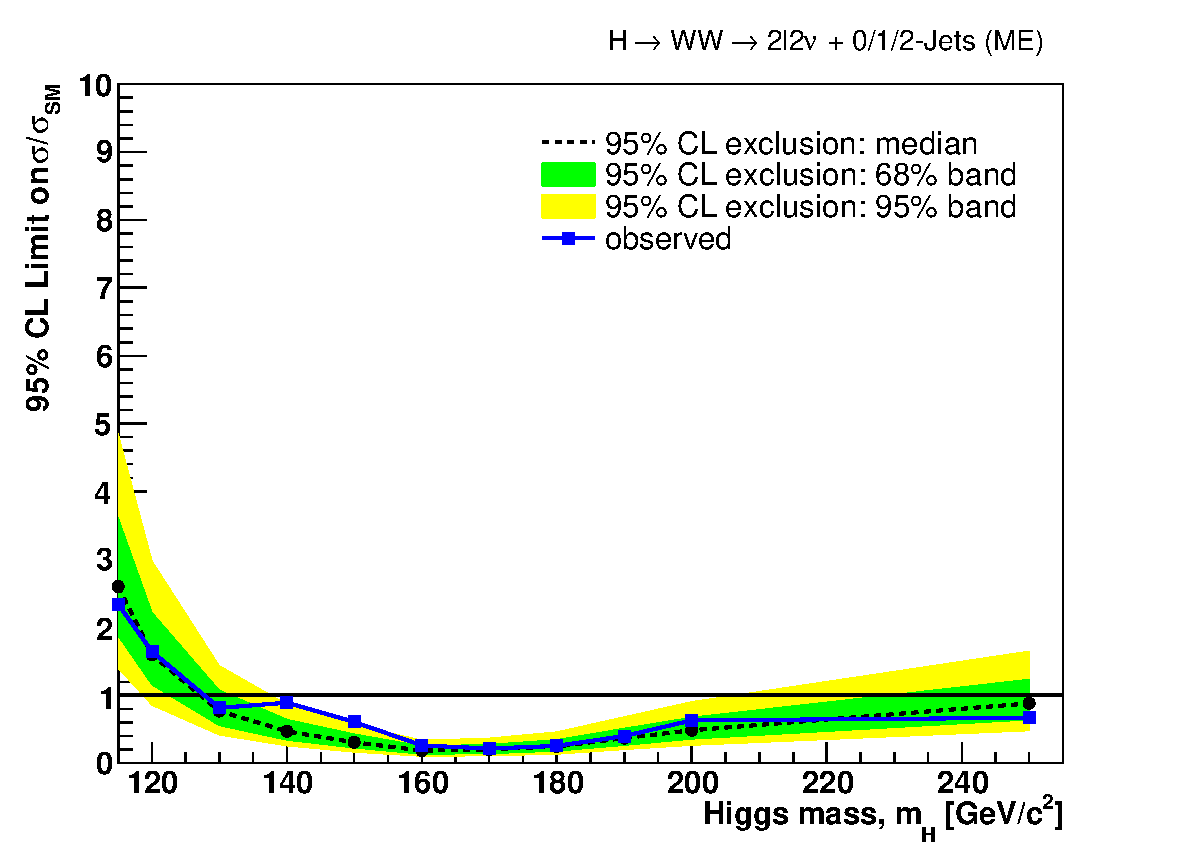
\includegraphics[width=.45\textwidth]{figures/limit_nj_shape_me-CLs-asymptotic.pdf}}
\caption{ Shape analysis upper limits based on the BDT and matrix element outputs at 95\% C.L. for $\intlumi$ data. }
\label{fig:me_results_5fb}
\end{figure}
%%%%%%%%%%%%%%%%%%%%%%%%%%%%%%

%%%%%%%%%%%%%%%%%%%%%%%%%%%%%%
\begin{table}[!htbp]
\begin{center}
\begin{tabular}{c c c c c c}
\hline\hline
 Higgs Mass   & Observed & Median expected & Expected range for 68\% & Expected range for 95\%   \\
\hline
\multicolumn{5}{c} {BDT Based} \\
\hline
115 & 3.7 & 2.5 & [1.8, 3.5] & [1.4, 4.8] \\
120 & 2.4 & 1.5 & [1.1, 2.1] & [0.8, 2.8] \\
130 & 0.9 & 0.7 & [0.5, 1.0] & [0.4, 1.3] \\
140 & 0.6 & 0.4 & [0.3, 0.6] & [0.2, 0.8] \\
150 & 0.4 & 0.3 & [0.2, 0.4] & [0.2, 0.6] \\
160 & 0.3 & 0.2 & [0.1, 0.3] & [0.1, 0.4] \\
170 & 0.3 & 0.2 & [0.2, 0.3] & [0.1, 0.4] \\
180 & 0.3 & 0.3 & [0.2, 0.4] & [0.1, 0.5] \\
190 & 0.4 & 0.4 & [0.3, 0.6] & [0.2, 0.7] \\
200 & 0.5 & 0.5 & [0.4, 0.7] & [0.3, 1.0] \\
250 & 0.8 & 0.9 & [0.7, 1.3] & [0.5, 1.8] \\
300 & 1.0 & 1.0 & [0.7, 1.3] & [0.5, 1.8] \\
350 & 0.8 & 0.8 & [0.6, 1.2] & [0.5, 1.6] \\
400 & 1.0 & 0.9 & [0.7, 1.3] & [0.5, 1.7] \\
450 & 1.0 & 1.3 & [0.9, 1.7] & [0.7, 2.3] \\
500 & 1.2 & 1.7 & [1.2, 2.4] & [0.9, 3.2] \\
550 & 1.8 & 2.6 & [1.9, 3.6] & [1.4, 4.8] \\
600 & 2.2 & 3.6 & [2.6, 5.0] & [1.9, 6.7] \\
\hline
\multicolumn{5}{c} {Matrix Element Method} \\
\hline
115 & 2.4 & 2.6 & [1.9, 3.6] & [1.4, 4.8] \\
120 & 1.6 & 1.6 & [1.1, 2.2] & [0.9, 3.0] \\
130 & 0.8 & 0.8 & [0.6, 1.1] & [0.4, 1.4] \\
140 & 0.9 & 0.5 & [0.3, 0.6] & [0.2, 0.9] \\
150 & 0.5 & 0.3 & [0.2, 0.4] & [0.2, 0.6] \\
160 & 0.2 & 0.2 & [0.1, 0.3] & [0.1, 0.3] \\
170 & 0.2 & 0.2 & [0.1, 0.3] & [0.1, 0.4] \\
180 & 0.3 & 0.2 & [0.2, 0.3] & [0.1, 0.5] \\
190 & 0.4 & 0.4 & [0.3, 0.5] & [0.2, 0.7] \\
200 & 0.6 & 0.5 & [0.4, 0.7] & [0.3, 0.9] \\
250 & 0.7 & 0.9 & [0.6, 1.2] & [0.5, 1.7] \\
300 & 0.9 & 1.0 & [0.7, 1.4] & [0.5, 1.9] \\
350 & 1.0 & 0.9 & [0.6, 1.2] & [0.5, 1.7] \\
400 & 0.7 & 1.0 & [0.7, 1.4] & [0.5, 1.8] \\
450 & 1.0 & 1.4 & [1.0, 1.9] & [0.7, 2.5] \\
500 & 1.4 & 1.9 & [1.4, 2.7] & [1.0, 3.6] \\
550 & 1.9 & 2.7 & [2.0, 3.8] & [1.5, 5.1] \\
600 & 2.8 & 4.1 & [2.9, 5.7] & [2.2, 7.6] \\
 \hline\hline
\end{tabular}
\end{center}
\caption{Multivariate shape analysis expected and observed upper limits at 95\% C.L.
for $\intlumi$ data using the BDT and matrix element outputs for the {\bf combined 0/1/2 jet bins}.}
\label{tab:me_results_5fb}
\end{table}
%%%%%%%%%%%%%%%%%%%%%%%%%%%%%%


%%%%%%%%%%%%%%%%%%%%%%%%%%%%%%
\begin{figure}[!hbtp]
\centering
\subfigure[BDT 0-Jet SF]{
\centering
\label{subfig:bdt_0jsf}
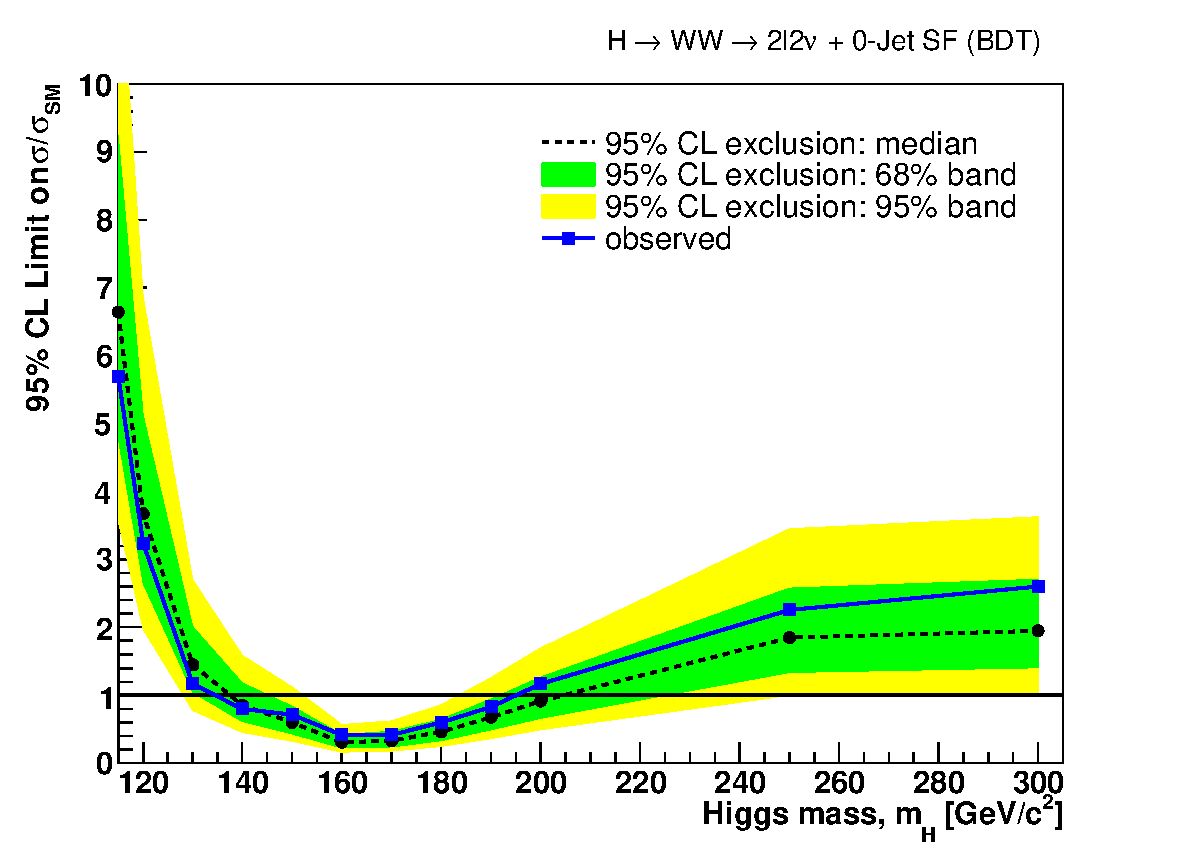
\includegraphics[width=.42\textwidth]{figures/limit_0jsf_shape_bdt-CLs-asymptotic.pdf}}
\subfigure[ME 0-Jet SF]{
\centering
\label{subfig:me_0jsf}
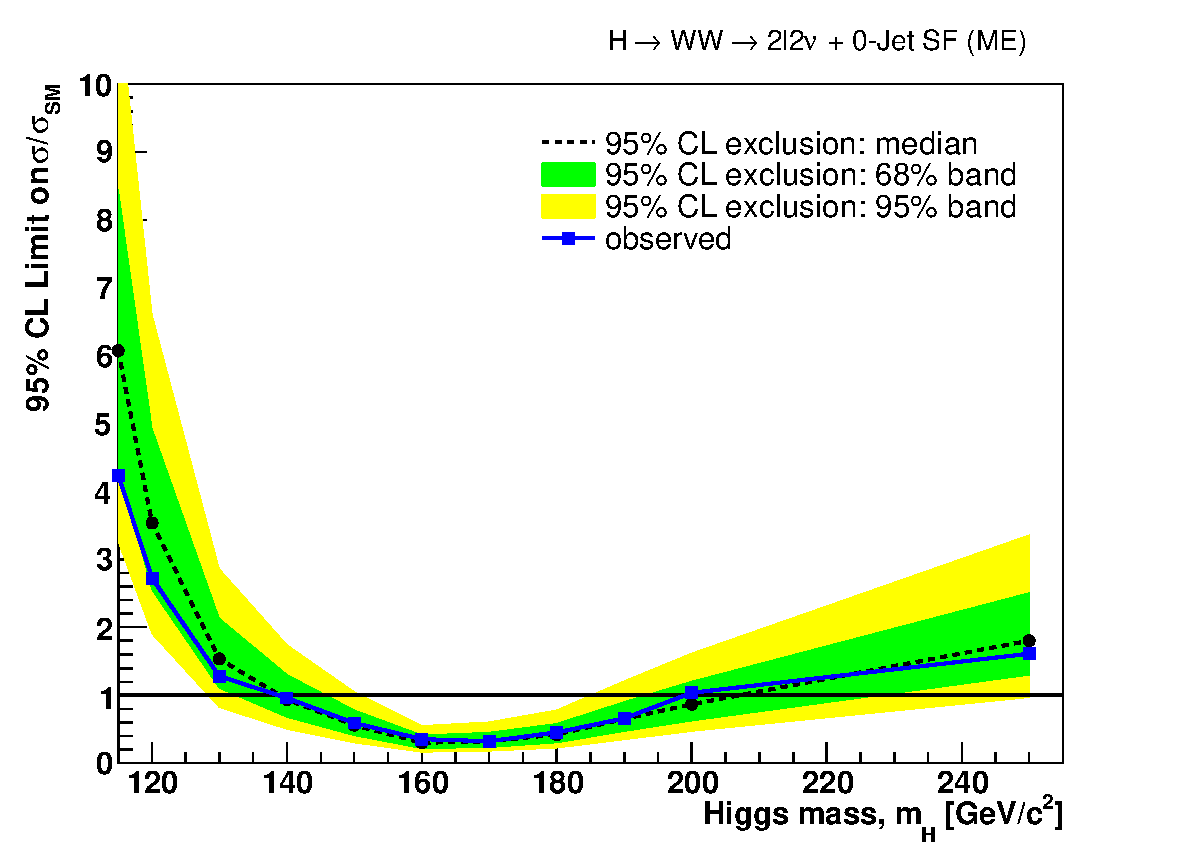
\includegraphics[width=.42\textwidth]{figures/limit_0jsf_shape_me-CLs-asymptotic.pdf}}
\centering
\subfigure[BDT 0-Jet OF]{
\centering
\label{subfig:bdt_0jof}
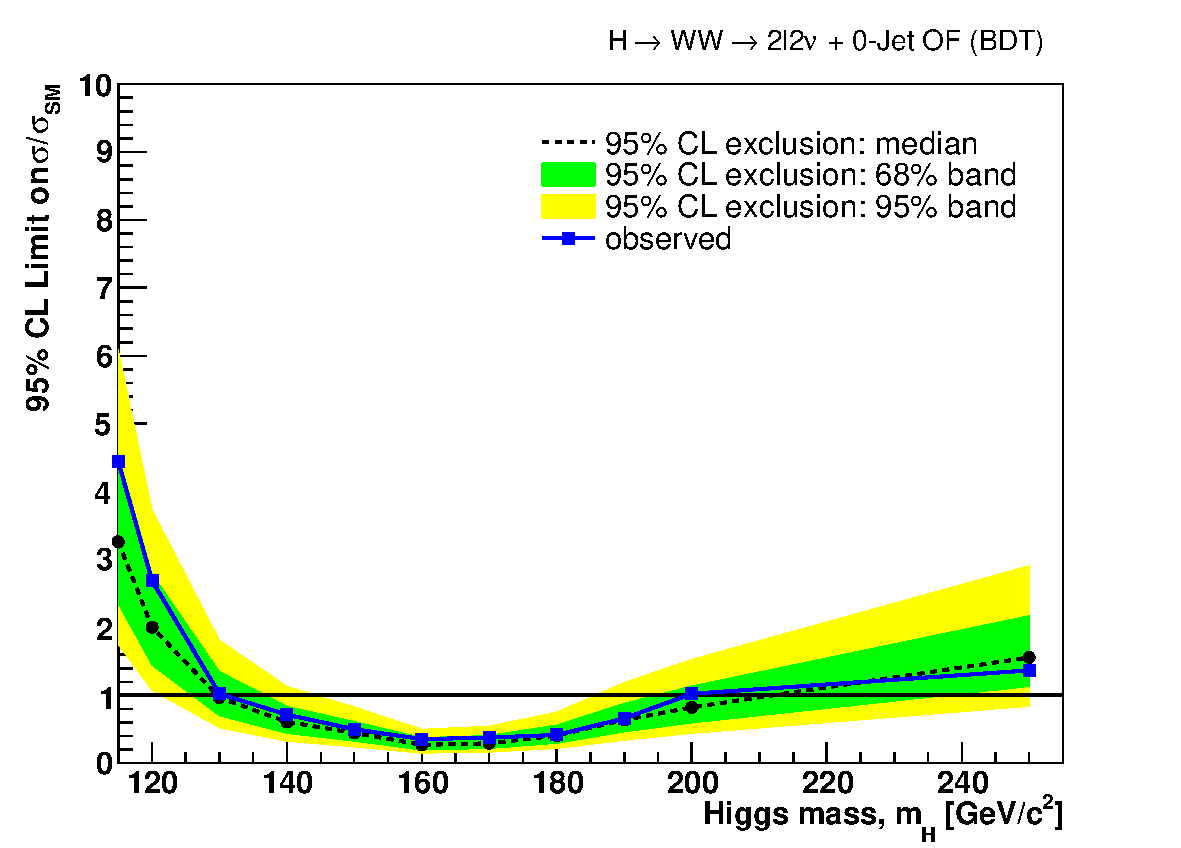
\includegraphics[width=.42\textwidth]{figures/limit_0jof_shape_bdt-CLs-asymptotic.pdf}}
\subfigure[ME 0-Jet OF]{
\centering
\label{subfig:me_0jof}
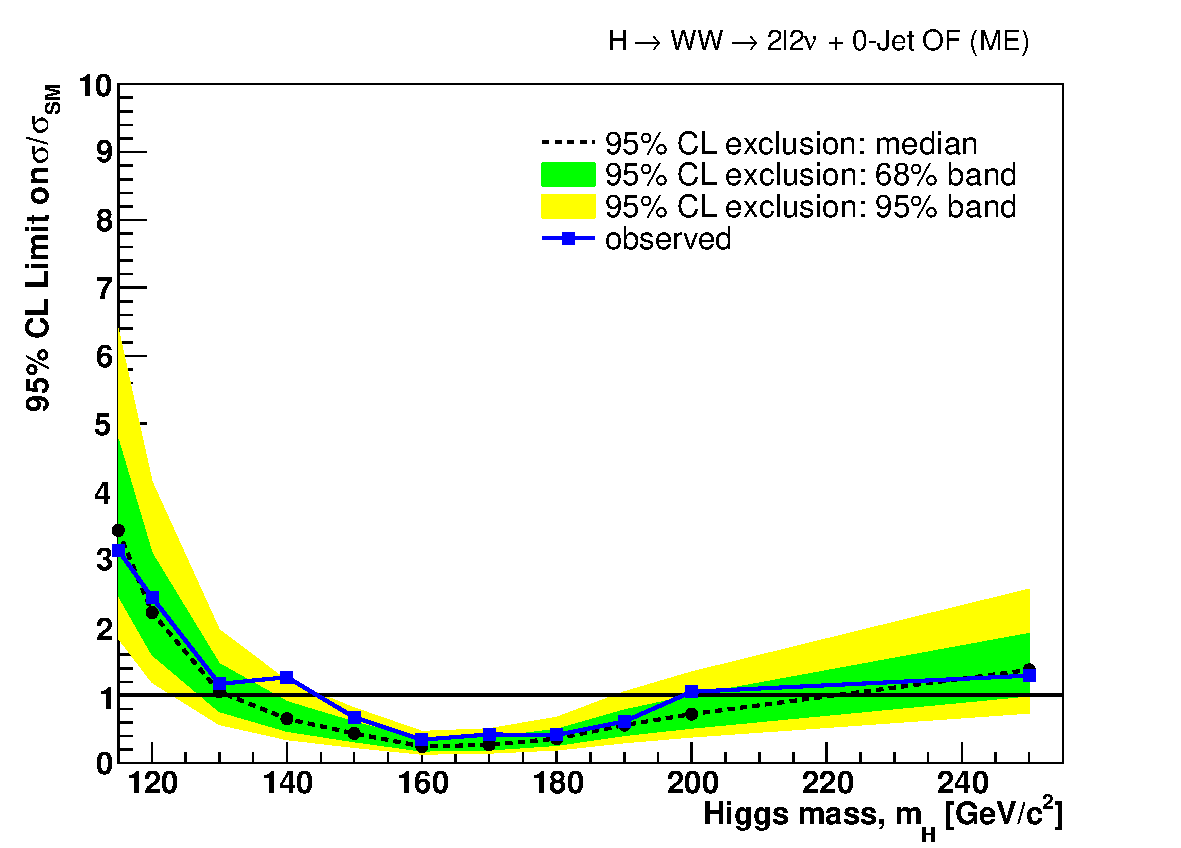
\includegraphics[width=.42\textwidth]{figures/limit_0jof_shape_me-CLs-asymptotic.pdf}}
\centering
\subfigure[BDT 1-Jet SF]{
\centering
\label{subfig:bdt_1jsf}
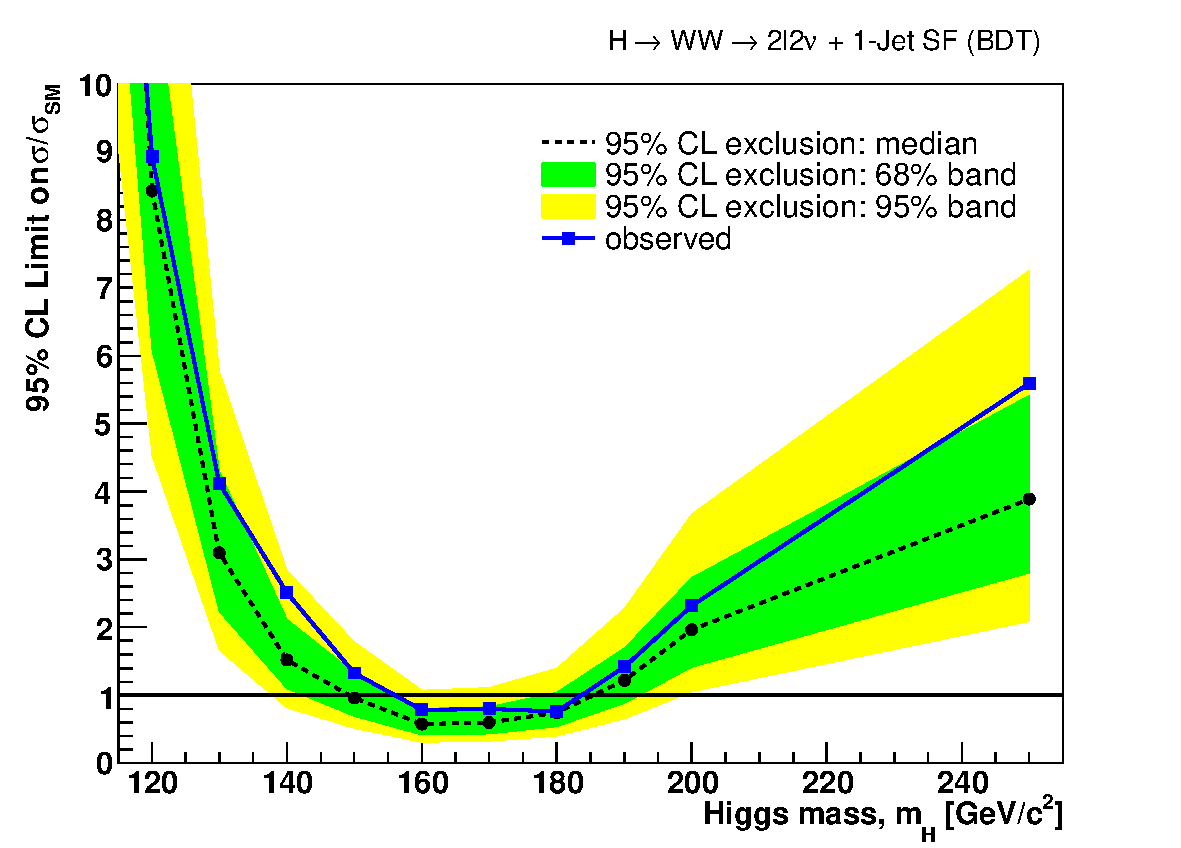
\includegraphics[width=.42\textwidth]{figures/limit_1jsf_shape_bdt-CLs-asymptotic.pdf}}
\subfigure[ME 1-Jet SF]{
\centering
\label{subfig:me_1jsf}
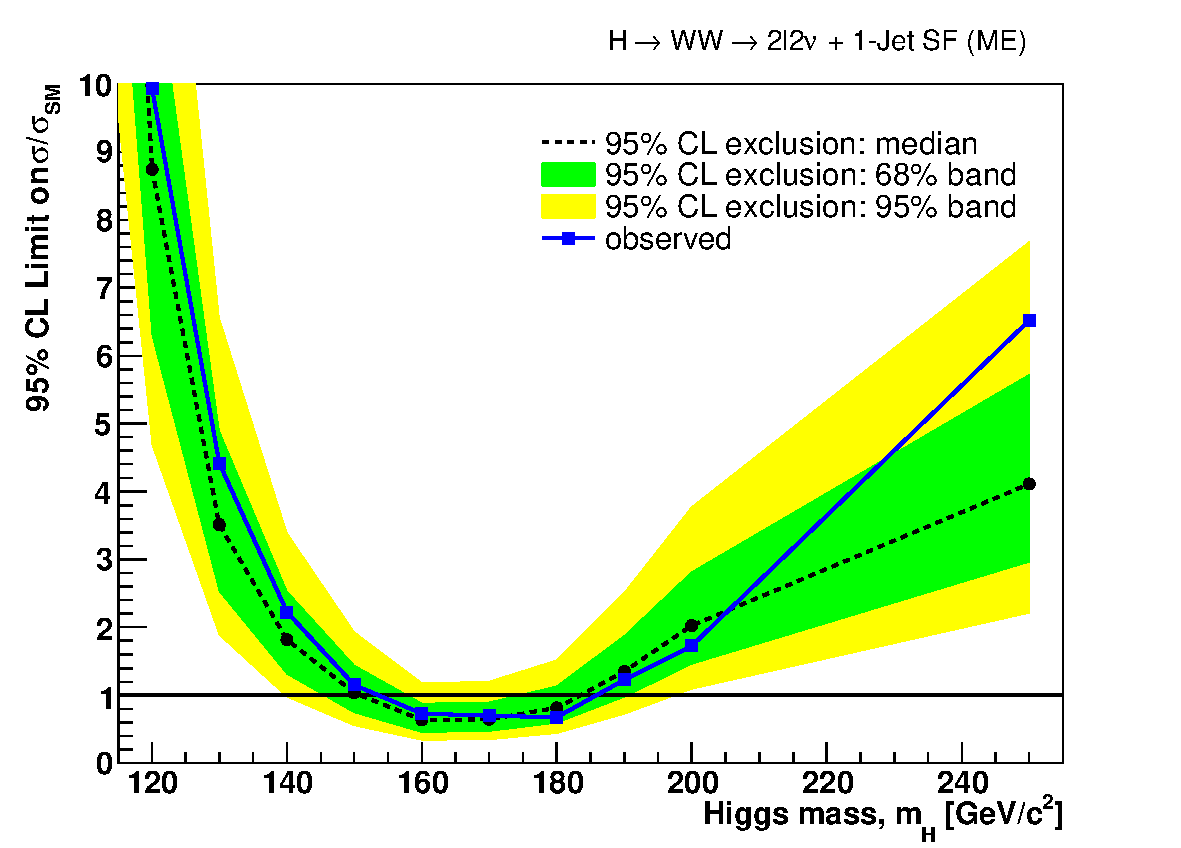
\includegraphics[width=.42\textwidth]{figures/limit_1jsf_shape_me-CLs-asymptotic.pdf}}
\centering
\subfigure[BDT 1-Jet OF]{
\centering
\label{subfig:bdt_1jof}
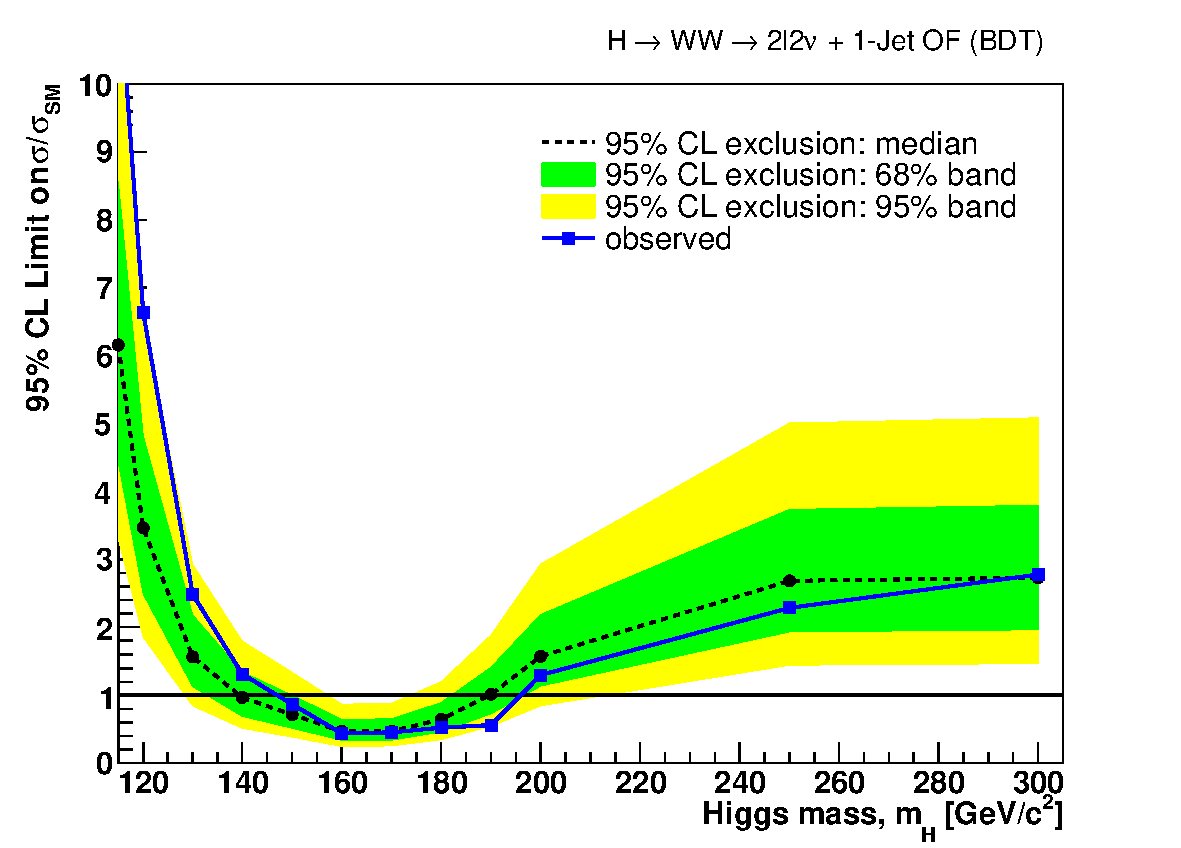
\includegraphics[width=.42\textwidth]{figures/limit_1jof_shape_bdt-CLs-asymptotic.pdf}}
\subfigure[ME 1-Jet OF]{
\centering
\label{subfig:me_1jof}
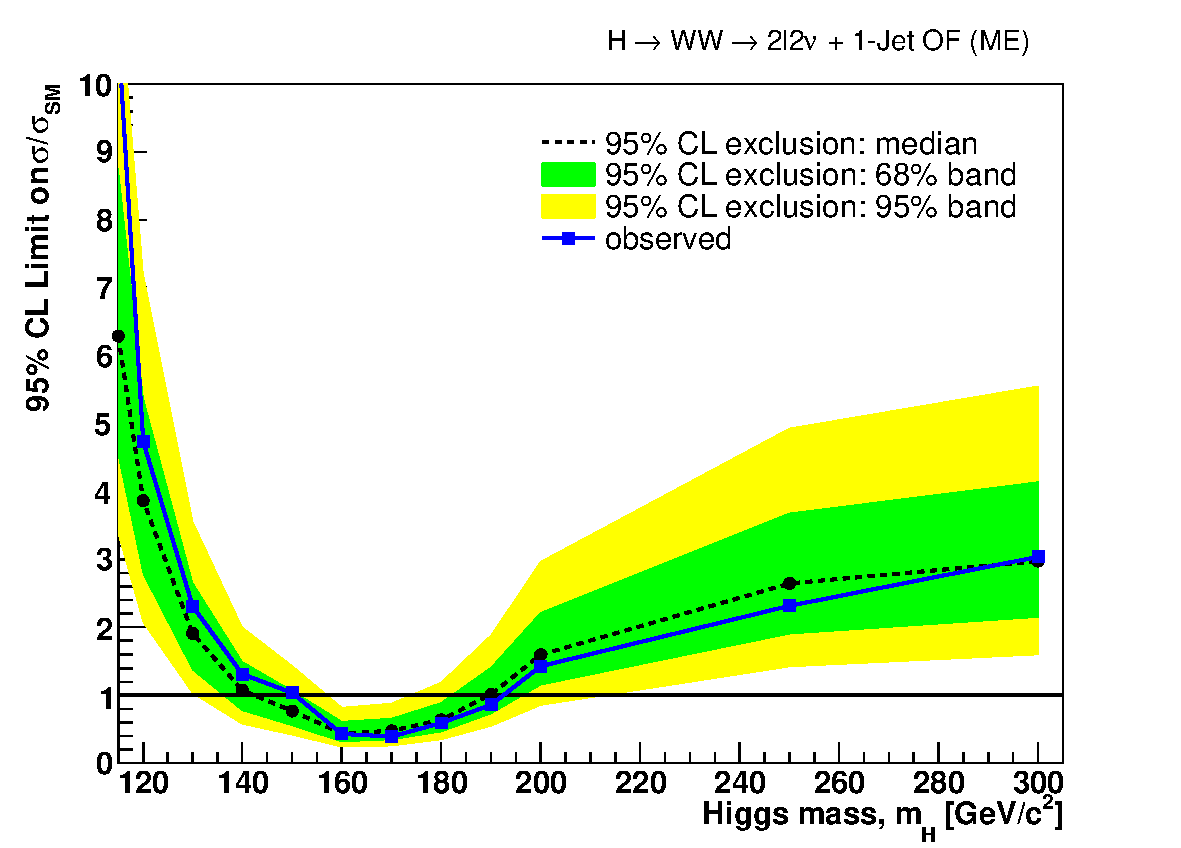
\includegraphics[width=.42\textwidth]{figures/limit_1jof_shape_me-CLs-asymptotic.pdf}}
\caption{ Shape analysis upper limits based on the BDT and matrix element outputs at 95\% C.L. for $\intlumi$ data. 
Limits are presented separately for the 4 sub-channels for each method. }
%1) 0-Jet bin same flavor; 2) 0-Jet bin opposite flavor; 3) 1-Jet bin same flavor; 4) 1-Jet bin opposite flavor.}
\label{fig:me_results_5fb_subchannel}
\end{figure}
%%%%%%%%%%%%%%%%%%%%%%%%%%%%%%


%%%%%%%%%%%%%%%%%%%%%%%%%%%%%%
%\begin{table}[!htbp]
%\begin{center}
%\begin{tabular}{c c c c c c}
%\hline\hline
% Higgs Mass   & Observed & Median expected & Expected range for 68\% & Expected range for 95\%   \\
%\hline
%\multicolumn{5}{c} {BDT Based} \\
%\hline
%115 & 3.6 & 3.2 & [2.2, 4.8] & [1.5, 7.0] \\
%120 & 2.4 & 1.8 & [1.2, 2.7] & [0.9, 4.0] \\
%130 & 0.9 & 0.9 & [0.6, 1.3] & [0.4, 1.8] \\
%140 & 0.6 & 0.5 & [0.3, 0.8] & [0.2, 1.1] \\
%150 & 0.5 & 0.4 & [0.2, 0.5] & [0.2, 0.8] \\
%160 & 0.3 & 0.2 & [0.1, 0.3] & [0.1, 0.4] \\
%170 & 0.4 & 0.2 & [0.1, 0.3] & [0.1, 0.5] \\
%180 & 0.4 & 0.3 & [0.2, 0.5] & [0.1, 0.7] \\
%190 & 0.6 & 0.5 & [0.3, 0.7] & [0.2, 1.1] \\
%200 & 0.7 & 0.7 & [0.4, 1.0] & [0.3, 1.5] \\
%250 & 1.1 & 1.3 & [0.8, 2.0] & [0.5, 2.9] \\
%300 & 1.2 & 1.3 & [0.9, 2.0] & [0.6, 2.9] \\
%350 & 1.1 & 1.2 & [0.8, 1.8] & [0.5, 2.7] \\
%400 & 1.3 & 1.3 & [0.9, 2.1] & [0.6, 3.0] \\
%450 & 1.4 & 1.9 & [1.3, 2.9] & [0.8, 4.3] \\
%500 & 1.7 & 2.8 & [1.9, 4.3] & [1.3, 6.5] \\
%550 & 2.9 & 4.3 & [2.9, 6.6] & [1.9, 10.3] \\
%600 & 3.8 & 6.5 & [4.2, 10.2] & [2.8, 15.6] \\
%\hline
%\multicolumn{5}{c} {Matrix Element Method} \\
%\hline
%115 & 2.5 & 3.2 & [2.2, 4.8] & [1.5, 7.1] \\
%120 & 2.1 & 2.0 & [1.3, 3.0] & [0.9, 4.3] \\
%130 & 0.9 & 0.9 & [0.6, 1.4] & [0.4, 2.0] \\
%140 & 1.0 & 0.6 & [0.4, 0.9] & [0.2, 1.2] \\
%150 & 0.6 & 0.4 & [0.2, 0.5] & [0.2, 0.8] \\
%160 & 0.3 & 0.2 & [0.1, 0.3] & [0.1, 0.4] \\
%170 & 0.3 & 0.2 & [0.1, 0.3] & [0.1, 0.4] \\
%180 & 0.4 & 0.3 & [0.2, 0.4] & [0.1, 0.6] \\
%190 & 0.5 & 0.4 & [0.3, 0.7] & [0.2, 0.9] \\
%200 & 0.9 & 0.6 & [0.4, 0.9] & [0.3, 1.3] \\
%250 & 0.9 & 1.2 & [0.8, 1.8] & [0.5, 2.6] \\
%300 & 1.1 & 1.4 & [0.9, 2.1] & [0.6, 3.1] \\
%350 & 1.2 & 1.2 & [0.8, 1.9] & [0.6, 2.8] \\
%400 & 1.1 & 1.4 & [0.9, 2.1] & [0.6, 3.2] \\
%450 & 1.3 & 2.1 & [1.4, 3.2] & [0.9, 4.8] \\
%500 & 2.3 & 3.2 & [2.2, 4.9] & [1.5, 7.4] \\
%550 & 3.0 & 4.9 & [3.3, 7.7] & [2.2, 11.7] \\
%600 & 5.0 & 7.8 & [5.0, 12.1] & [3.3, 19.2] \\
%\hline\hline
%\end{tabular}
%\end{center}
%\caption{Multivariate shape analysis expected and observed upper limits at 95\% C.L.
%for $\intlumi$ data using the BDT and matrix element outputs for the {\bf 0-jet bin}.}
%\label{tab:me_results_5fb_0j}
%\end{table}
%%%%%%%%%%%%%%%%%%%%%%%%%%%%%%

%%%%%%%%%%%%%%%%%%%%%%%%%%%%%%
%\begin{table}[!htbp]
%\begin{center}
%\begin{tabular}{c c c c c c}
%\hline\hline
% Higgs Mass   & Observed & Median expected & Expected range for 68\% & Expected range for 95\%   \\
%\hline
%\multicolumn{5}{c} {BDT Based} \\
%\hline
%115 & 6.1 & 7.8 & [5.3, 11.9] & [3.8, 18.3] \\
%120 & 3.5 & 4.0 & [2.7, 6.1] & [1.9, 9.1] \\
%130 & 1.4 & 1.5 & [1.0, 2.2] & [0.7, 3.3] \\
%140 & 0.8 & 0.9 & [0.6, 1.3] & [0.4, 1.8] \\
%150 & 0.8 & 0.6 & [0.4, 0.9] & [0.3, 1.3] \\
%160 & 0.5 & 0.3 & [0.2, 0.4] & [0.1, 0.6] \\
%170 & 0.4 & 0.3 & [0.2, 0.5] & [0.2, 0.7] \\
%180 & 0.6 & 0.5 & [0.3, 0.7] & [0.2, 1.0] \\
%190 & 0.9 & 0.7 & [0.5, 1.0] & [0.3, 1.5] \\
%200 & 1.3 & 1.0 & [0.7, 1.5] & [0.5, 2.3] \\
%250 & 2.2 & 2.1 & [1.4, 3.1] & [1.0, 4.3] \\
%\hline
%\multicolumn{5}{c} {Matrix Element Method} \\
%\hline
%115 & 4.1 & 7.6 & [5.1, 12.3] & [3.6, 19.2] \\
%120 & 2.8 & 4.3 & [2.8, 6.2] & [2.0, 9.3] \\
%130 & 1.3 & 1.6 & [1.1, 2.4] & [0.7, 3.6] \\
%140 & 0.9 & 1.0 & [0.7, 1.5] & [0.4, 2.2] \\
%150 & 0.7 & 0.6 & [0.4, 0.9] & [0.3, 1.3] \\
%160 & 0.4 & 0.3 & [0.2, 0.4] & [0.1, 0.6] \\
%170 & 0.3 & 0.3 & [0.2, 0.5] & [0.1, 0.7] \\
%180 & 0.5 & 0.4 & [0.3, 0.6] & [0.2, 0.9] \\
%190 & 0.7 & 0.7 & [0.5, 1.0] & [0.3, 1.5] \\
%200 & 1.1 & 0.9 & [0.6, 1.4] & [0.4, 2.0] \\
%250 & 1.6 & 1.9 & [1.3, 2.9] & [0.9, 4.4] \\
%\hline\hline
%\end{tabular}
%\end{center}
%\caption{Multivariate shape analysis expected and observed upper limits at 95\% C.L.
%for $\intlumi$ data using the BDT and matrix element outputs for {\bf 1 jet bin}.}
%\label{tab:me_results_5fb_1j}
%\end{table}
%%%%%%%%%%%%%%%%%%%%%%%%%%%%%%

%
